\documentclass[12pt]{report}
\usepackage{report}

\usepackage[acronym]{glossaries}
\usepackage{rotating}
\usepackage{float}
\usepackage{siunitx}
\usepackage{array}
\usepackage[justification=centering]{caption}
\captionsetup[figure]{font=small}
\usepackage{booktabs}
\usepackage[table,xcdraw]{xcolor}
\usepackage{chngcntr}
\usepackage[utf8]{inputenc}
\usepackage{listings}
\usepackage{subcaption}
\usepackage{indentfirst}
\usepackage{enumitem}
\usepackage{booktabs}
\usepackage{multirow}
\usepackage{flafter}
\usepackage{hyperref}
\usepackage{minted}
\usepackage{fontspec}
 
\setmainfont{Times New Roman}

\hypersetup{
    colorlinks=true,
    linkcolor=blue,
    filecolor=magenta,      
    urlcolor=blue,
    pdftitle={LMS Integration with Namaste BHU},
    pdfpagemode=FullScreen,
}


\setcounter{secnumdepth}{3} % for subheadings
\setlength{\cfttabindent}{0pt} %for tables
\setlength{\cftfigindent}{0pt} %for figures


\title{LMS Integration with Namaste BHU}
\author{Pradyumna Krishna}
\date{\today}
\counterwithout{figure}{section}
\counterwithin{figure}{chapter}
\counterwithout{table}{section}
\counterwithin{table}{chapter}

\begin{document}
\addtocontents{toc}{\protect Title \hfill Page No.\par \bigskip}

\thispagestyle{empty} % This will hide pagenumber in title page
\tolerance=1
\emergencystretch=\maxdimen
\hyphenpenalty=10000
\hbadness=10000

% First title page
\begin{titlepage}
{
	\thispagestyle{empty}
	\centering
	\large

    \vspace*{0cm}
	\textbf{\LARGE LMS Integration with Namaste BHU}
    \\[0.5cm]
    \textit{A Minor-Project report submitted in partial fulfillment of the requirements for the award of the degree of}
	\\[1.5cm]
    \textbf{Master of Computer Science}
    \\[1.5cm]
    by
    \\[1.5cm]
    {\bf Pradyumna Krishna}\\
    {\bf (22419CMP020)}\\[1.5cm]
    
    
\includegraphics[width=1.5in]{assets/img/emblem.png}
    \vspace*{\fill}

    \bf \Large
    Department of Computer Science\\
    Institute of Science\\
    \LARGE
    Banaras Hindu University, Varanasi - 221005\\
    \Large
    2024\\[1.5cm]
}
\end{titlepage}



\pagenumbering{roman} % roman page numbers


%% This is constant for all the reports 
\newpage
\chapter*{ABSTRACT}
\addcontentsline{toc}{section}{ABSTRACT}

The integration of a Learning Management System (LMS) with the Namaste BHU application represents a significant advancement in the digital infrastructure of Banaras Hindu University (BHU). This project aims to seamlessly connect Moodle, an open-source LMS, with the Namaste BHU application to create a unified platform for academic management, communication, and engagement. The project encompasses deployment, configuration, and integration phases, involving the setup of Moodle on an Azure instance, updates to the Namaste BHU application, and the development of custom plugins and extensions. Through single sign-on (SSO), deep linking, and notification delivery mechanisms, users can access Moodle content directly from the Namaste BHU application, receive real-time updates and announcements, and collaborate effectively within the academic community. The successful completion of this project signifies a significant milestone in enhancing the academic experience at BHU, promoting accessibility, efficiency, and innovation in teaching and learning practices. Future opportunities for enhancement and expansion include advanced analytics, personalized learning pathways, and integration with external tools and services, ensuring the continued evolution and relevance of the integrated platform in the digital age of education.

\emph{\textbf{Keywords}: Learning Management System (LMS), Namaste BHU, Moodle, Single Sign-On (SSO), Deep Linking}

% Acknowledgments

\newpage
\chapter*{ACKNOWLEDGEMENT}
\addcontentsline{toc}{section}{ACKNOWLEDGEMENT}

\normalsize
I would like to express my deepest gratitude to my supervisor,\textbf{ Dr. T.V. Prabhakar}, for his invaluable guidance, mentorship, and unwavering support throughout the duration of this project. Dr. Prabhakar's expertise, insights, and encouragement have been instrumental in shaping the direction and execution of the LMS Integration with Namaste BHU project. His dedication to academic excellence and commitment to my growth as a researcher have been truly inspiring, and I am profoundly grateful for the opportunity to learn from him.

I would also like to extend my heartfelt thanks to \textbf{Dev Angiras} for his constant support and invaluable assistance at every stage of the project. Dev's deep understanding of the Namaste BHU architecture, system architecture, and attention to detail have been instrumental in navigating the complexities of integration and ensuring the seamless functioning of the integrated platform. His tireless efforts, patience, and collaborative spirit have been indispensable, and I am immensely grateful for his unwavering dedication.




{
\hypersetup{linkcolor=black}
% Table of contents
{
\begin{center}
  \setlength{\parskip}{0em}
  \renewcommand\contentsname{TABLE OF CONTENTS} % This will change heading text
  \tableofcontents %\addcontentsline{toc}{section}{TABLE OF CONTENTS}
\end{center}
}

% List of figures - if any

\newpage
\listoffigures 
\addcontentsline{toc}{section}{LIST OF FIGURES}

% List of tables- if any

\newpage
\listoftables 
\addcontentsline{toc}{section}{LIST OF TABLES}
}


\newpage
\newpage
\pagenumbering{arabic}
\chapter{INTRODUCTION}


% \clearpage

\section{Background}

Namaste BHU serves as a comprehensive digital platform catering to the needs of students, faculty, and staff within Banaras Hindu University (BHU). Its multifaceted features, ranging from simplified course syllabi to centralized notice boards, aim to streamline campus life, foster engagement, and provide timely information to the university community.

A Learning Management System (LMS) is a digital platform designed to facilitate the administration, documentation, tracking, reporting, and delivery of educational courses or training programs. In the context of modern education, LMS has become indispensable, offering a centralized hub for course materials, assessments, communication tools, and more.

The integration of LMS with Namaste BHU presents a compelling opportunity to enhance the academic experience and communication channels within the university ecosystem. By combining the robust features of an LMS with the convenience and accessibility of Namaste BHU, students, faculty, and staff can benefit from a cohesive digital environment that streamlines various aspects of teaching, learning, and administrative processes.

\section{Motivation}
The integration of LMS with Namaste BHU is motivated by a desire to address the challenges faced by the university community in managing various academic activities and communication channels. The motivation can be explained as follows:

\begin{enumerate}
    \item \textbf{Need for Seamless Academic Management}:
    Recognizing the challenges faced by students, faculty, and staff in managing various academic activities such as accessing course materials, communicating effectively, and staying updated with important announcements.
    \item \textbf{Streamlining Administrative Processes}:
    Enhance efficiency in managing academic-related processes, such as course registrations, grading, and feedback mechanisms.\\
    \item \textbf{Facilitating Communication}:
    Enable effective communication channels between students and faculty members through integrated messaging systems or discussion forums. Foster collaboration and engagement among users by facilitating peer-to-peer communication within the platform.
\end{enumerate}

\section{Consideration during Integration}
As the integration of an LMS with Namaste BHU represents a significant endeavor aimed at enhancing the academic experience and administrative efficiency within Banaras Hindu University (BHU), it is imperative to carefully consider various factors throughout the integration process. These considerations encompass technical, organizational, and user-centric aspects to ensure the successful implementation of the integrated platform. The following subsections outline key considerations that merit attention during the integration process:

\begin{enumerate}
	\item \textbf{Technical Compatibility}: Ensuring compatibility between the LMS software and the existing infrastructure of Namaste BHU, including server configurations, databases, and programming languages.
	\item \textbf{User Authentication and Access Control}: Implementing secure authentication mechanisms to ensure that users can access the integrated platform seamlessly using their existing credentials from Namaste BHU.
    \item \textbf{Security and Privacy}: Implementing robust security measures to protect sensitive academic and personal information shared within the integrated platform, including data encryption, secure transmission protocols, and authentication mechanisms.
    \item \textbf{Customization and Extension}: Providing flexibility for customization and extension of the integrated platform to accommodate specific requirements, workflows, and preferences of users within the university community. Developing APIs and integration points to enable seamless integration with third-party tools, services, and plugins.
	      	
\end{enumerate}

% \subsection{Scope of Project}

\newpage
\chapter{LITERATURE REVIEW}

\section{Learning Management System (LMS)}

A Learning Management System (LMS) is a software application or platform designed to facilitate the administration, delivery, and management of educational content and training programs. LMSs serve as centralized platforms for organizing course materials, facilitating communication between instructors and learners, tracking learner progress, and assessing performance.

The core features of an LMS typically include course creation and management tools, content authoring capabilities, communication and collaboration tools (such as discussion forums and messaging systems), assessment and grading functionalities, and reporting and analytics features. LMSs may also support integration with external systems and services, such as content repositories, authentication systems, and learning analytics tools.

The adoption of LMSs in educational institutions and corporate training environments has grown significantly in recent years, driven by the increasing demand for online learning solutions, the need for centralized management of digital resources, and the desire to enhance learner engagement and outcomes. LMSs offer flexibility, scalability, and accessibility, enabling organizations to deliver personalized and interactive learning experiences to diverse audiences.

\textbf{Core Features and Key Functionalities of an LMS}

\textbf{Course Management}\\
LMSs allow administrators and instructors to create, organize, and manage courses, including adding course materials, assignments, quizzes, and assessments.

\textbf{User Management}\\
LMSs enable the creation and management of user accounts, including students, instructors, administrators, and other stakeholders. User roles and permissions can be defined to control access to courses and content.

\textbf{Content Delivery}\\
LMSs provide tools for delivering educational content to users, such as multimedia presentations, documents, videos, and interactive modules. Content can be organized into modules or units for sequential learning.

\textbf{Communication and Collaboration}\\
LMSs offer communication and collaboration tools, such as discussion forums, messaging systems, and video conferencing, to facilitate interaction and engagement among users.

\textbf{Assessment and Evaluation}
LMSs support the creation, administration, and grading of quizzes, exams, assignments, and other assessments. They also provide tracking and reporting capabilities to monitor student progress and performance.


\section{System Design and Architecture}

Integrating an existing LMS into an existing ecosystem, such as the Namaste BHU application, requires careful consideration of system design and architecture techniques to ensure seamless communication, interoperability, and scalability. Several approaches and strategies can be employed to achieve successful integration:

\textbf{Service-Oriented Architecture (SOA)}

SOA is a design paradigm that advocates for the decomposition of complex systems into modular, interoperable services. By encapsulating LMS functionalities as independent services with well-defined interfaces, organizations can facilitate integration with external systems and applications, such as the Namaste BHU ecosystem. SOA promotes flexibility, reusability, and maintainability, allowing organizations to adapt to changing requirements and environments.

\textbf{API-Based Integration}

API-based integration involves exposing LMS functionalities and data through Application Programming Interfaces (APIs) that can be accessed and manipulated by external systems. By defining and implementing standardized APIs for course management, user authentication, content delivery, and other key functionalities, organizations can enable seamless communication and interaction between the LMS and the Namaste BHU application. API-based integration promotes interoperability, extensibility, and compatibility, allowing organizations to leverage the full potential of both systems.

\textbf{Middleware Solutions}

Middleware solutions, such as enterprise service buses (ESBs) or integration platforms as a service (iPaaS), can facilitate communication and data exchange between heterogeneous systems and applications. By deploying middleware solutions that support protocol translation, message routing, and data transformation, organizations can overcome interoperability challenges and streamline the integration process. Middleware solutions provide a centralized and scalable infrastructure for managing integrations, enabling organizations to achieve real-time data synchronization and seamless user experiences.

\textbf{Data Integration Techniques}

Data integration techniques, such as Extract, Transform, Load (ETL) processes, can be employed to synchronize and harmonize data between the LMS and the Namaste BHU application. By establishing data mappings, transformation rules, and synchronization schedules, organizations can ensure the consistency, accuracy, and integrity of data across both systems. Data integration techniques enable organizations to leverage data-driven insights and analytics for informed decision-making and personalized learning experiences.


\clearpage
\chapter{PROPOSED WORK AND METHODOLOGY}
\section{Current Architecture}
The existing architecture of the Namaste BHU application is straightforward, comprises a comprehensive framework that encompasses web server components, a mobile application interface, a centralized database, and integration with Firebase for notifications. This architecture is designed to provide a seamless and user-friendly experience for students, faculty, and staff at Banaras Hindu University (BHU).

\begin{figure}[h]
    \centering
    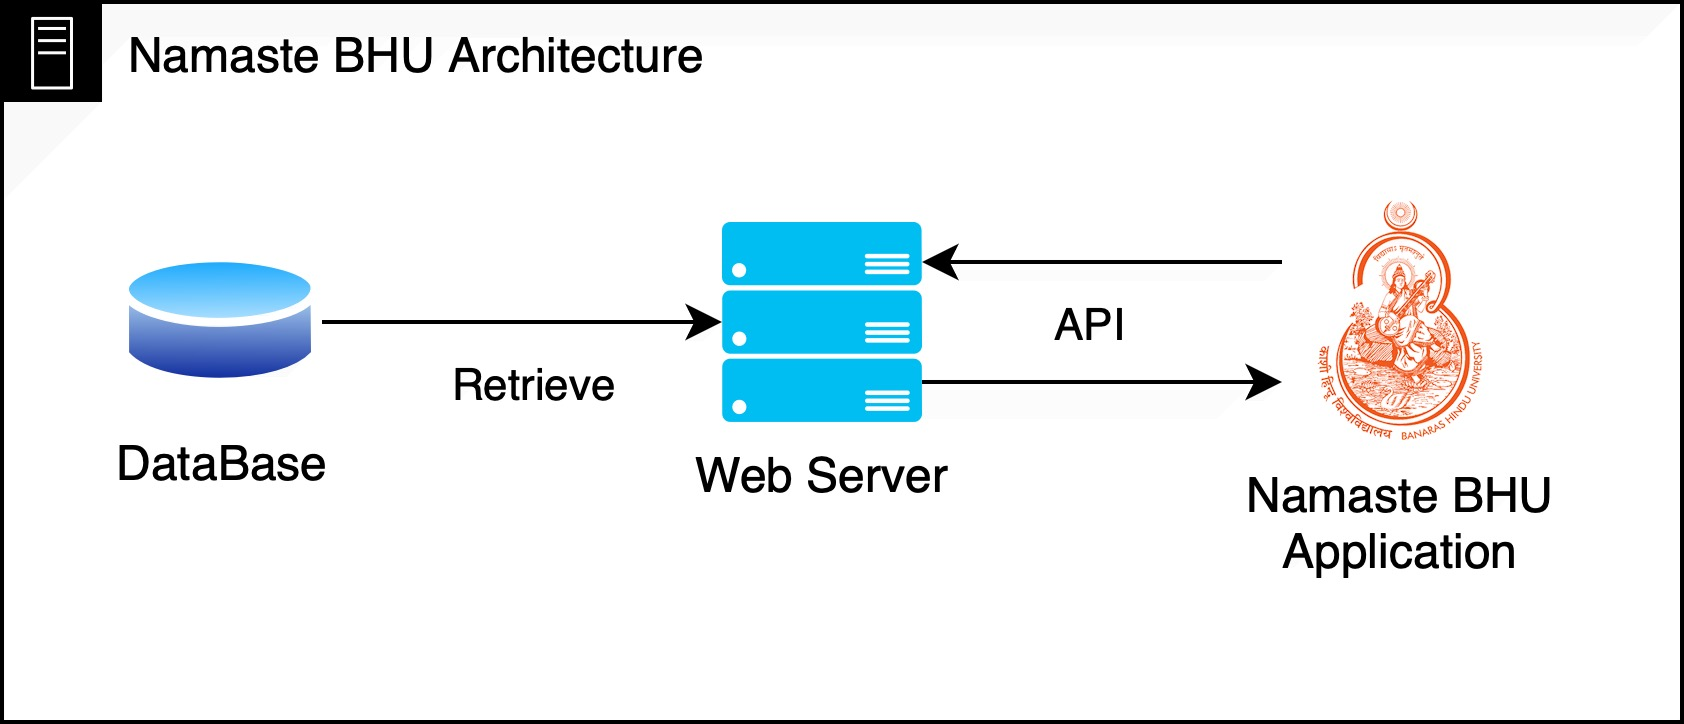
\includegraphics[width=0.75\linewidth]{assets/img/namaste-arch.jpg}
    \caption{Namaste BHU Architecture}
    \label{fig:namaste-arch}
\end{figure}

\textbf{Web Server}\\
The Namaste BHU web server components form the backbone of the application, serving as the centralized hub for managing and delivering various features and functionalities. The web server facilitates the exchange of data between the client-side interfaces (web and mobile) and the backend database, ensuring real-time updates and synchronization of information.

\textbf{Mobile Application}\\
The Namaste BHU mobile application serves as the primary access point for users to interact with the application on their mobile devices. It provides a user-friendly interface that enables students, faculty, and staff to access course materials, receive notifications, view event schedules, and engage with other features of the platform.

\textbf{Database}\\
The centralized database forms the core repository of data for the Namaste BHU application, housing essential information related to courses, students, faculty, events, and administrative records.

\section{Possible Solutions}
The integration of an LMS with the existing architecture of the Namaste BHU application presents a significant opportunity to enhance the academic experience and administrative efficiency within Banaras Hindu University (BHU). Several possible solutions can be considered to achieve this integration, each with its unique advantages and considerations. The following outlines some of the potential approaches:

\subsection{Development of a Custom LMS}
One possible solution involves developing a custom Learning Management System (LMS) specifically tailored to the needs and requirements of Banaras Hindu University (BHU). This approach offers the advantage of creating a bespoke solution that seamlessly integrates with the existing Namaste BHU architecture, providing a cohesive and unified platform for managing academic activities.

\subsection{Integrating an existing LMS}
Another possible solution is to integrate an existing Learning Management System (LMS) with Namaste BHU, leveraging the capabilities and features of established LMS platforms to enhance the academic experience and administrative efficiency within the university.

\begin{table}[h]
    \centering
    \begin{tabular}{|p{0.14\textwidth}|p{.38\textwidth}|p{0.38\textwidth}|}
        \hline
        \textbf{Solution} & Development of a Custom LMS & Integrating an existing LMS \\
        \hline
        \textbf{Advantages} &
        \begin{itemize}[noitemsep,topsep=0pt,leftmargin=*]
            \item Tailored to BHU's specific needs
            \item Seamless integration with Namaste BHU
            \item Flexibility and Scalability
        \end{itemize} &
        \begin{itemize}[noitemsep,topsep=0pt,leftmargin=*]
            \item Ready-made solution
            \item Continuous updates and improvements
        \end{itemize}\\
        \hline
        \textbf{Challenges} &
        \begin{itemize}[noitemsep,topsep=0pt,leftmargin=*]
            \item Time and resources
            \item Technical complexity
            \item Maintenance and support
        \end{itemize} &
        \begin{itemize}[noitemsep,topsep=0pt,leftmargin=*]
            \item Compatibility and customization
            \item Training and user adoption
        \end{itemize}\\
        \hline
    \end{tabular}
    \caption{Comparing Approaches}
    \label{tab:approaches}
\end{table}

The above approaches to integrate LMS with Namaste BHU are summarized in the table \ref{tab:approaches} with their advantages and challenges. After careful consideration of various options for integrating a Learning Management System (LMS) with Namaste BHU, the solution to integrate an existing LMS was more feasible and Moodle, an open source LMS emerges as the preferred choice.


\section{Why Moodle?}
Moodle, an open-source LMS widely adopted in educational institutions worldwide, offers a robust set of features, flexibility, scalability, and a vibrant community of developers and users. The following factors contribute to the selection of Moodle for integration with Namaste BHU:

\begin{enumerate}
    \item \textbf{Open Source Platform}: Moodle is an open-source Learning Management System, providing flexibility, customization, and community support without the need for costly licensing fees.
    \item \textbf{Robust Feature Set}: Moodle offers a comprehensive set of features for course management, assessment, communication, collaboration, and reporting, catering to the diverse needs of educational institutions.
    \item \textbf{Scalability and Customization}: Moodle is highly scalable and can accommodate the growth of Banaras Hindu University's user base, courses, and content over time. Moodle allows for extensive customization through plugins, themes, and modules, enabling tailored solutions to meet BHU's specific requirements and preferences.
    \item \textbf{Integration Capabilities}: Moodle offers seamless integration with third-party systems and services, facilitating integration with Namaste BHU and other university applications.
    \item \textbf{Active Community}: Moodle boasts a vibrant and active community of developers, educators, and administrators who contribute to ongoing development, support, and innovation.
\end{enumerate}

\section{Moodle Architecture}
Moodle follows a modular architecture that comprises several key components working together to deliver its functionality. Moodle's architecture consists of several key components that work together to provide a flexible, scalable, and customizable learning management system. The following components form the foundation of Moodle's architecture:

\begin{figure}[h]
    \centering
    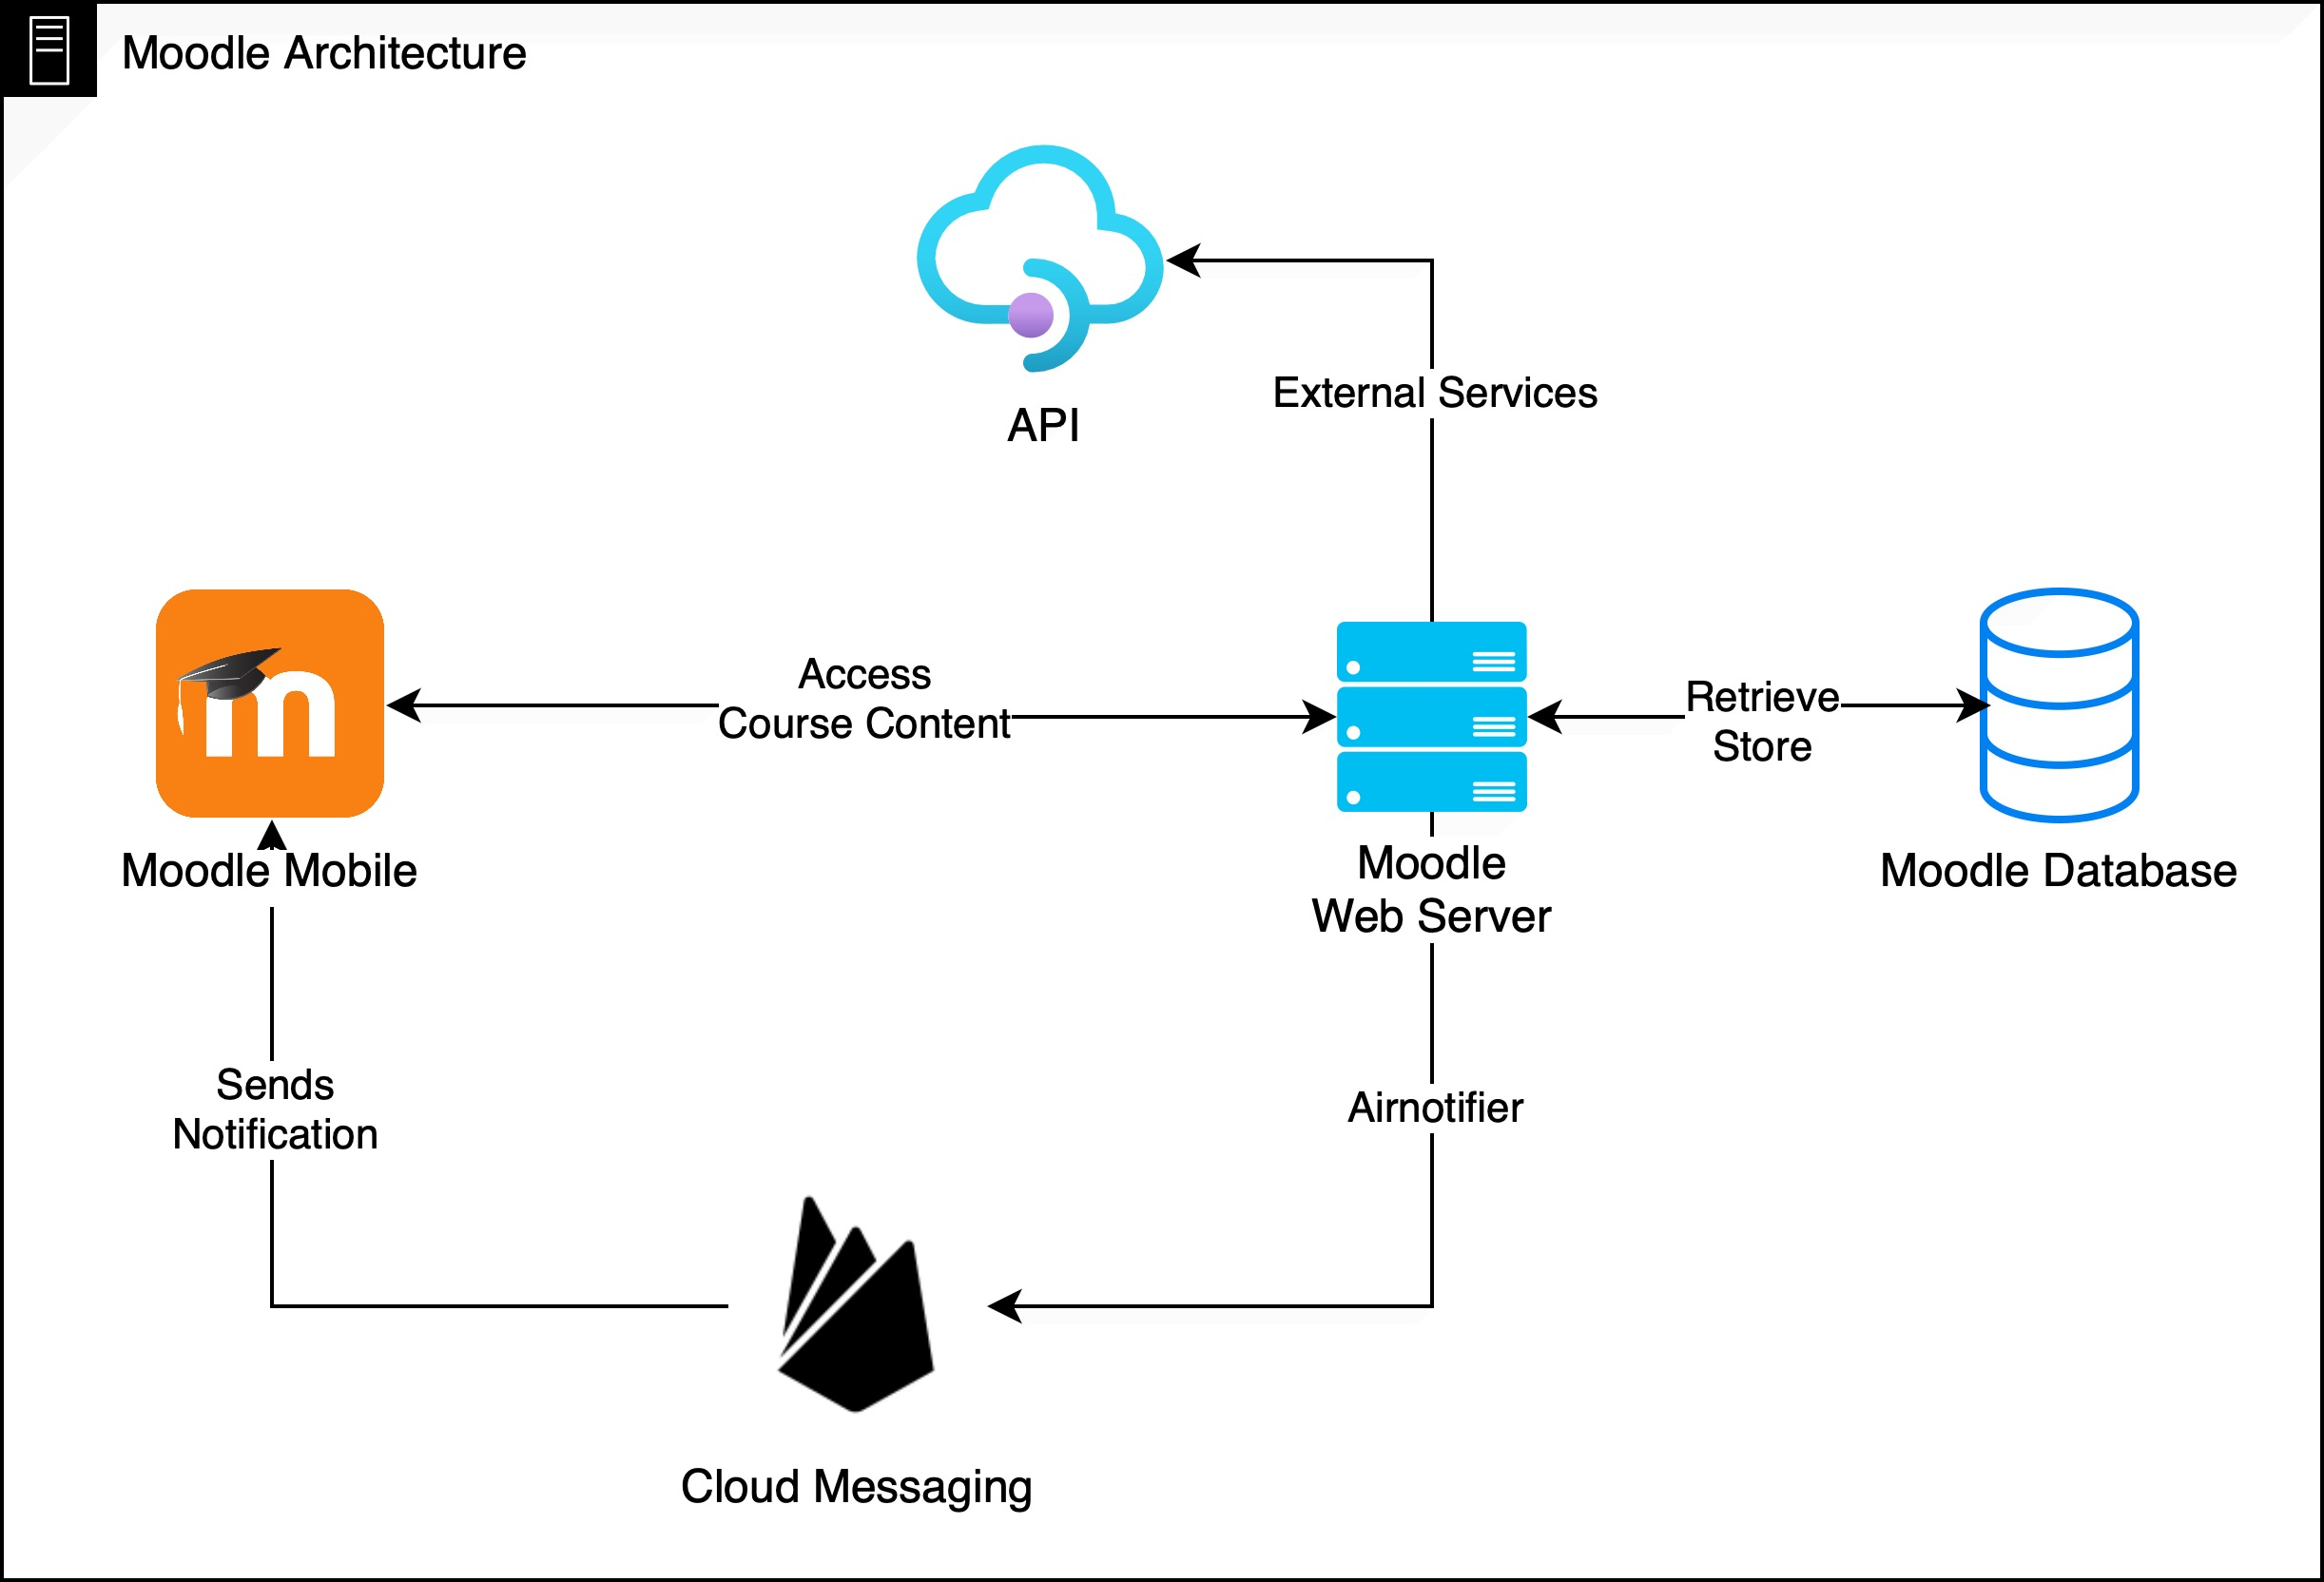
\includegraphics[width=0.75\linewidth]{assets/img/moodle-arch.jpg}
    \caption{Moodle Architecture}
    \label{fig:moodle-arch}
\end{figure}

\textbf{Web Server}\\
The web server component serves as the central point of access for users to interact with Moodle. It hosts the Moodle application and delivers web-based content, interfaces, and services to users across different devices and platforms.

\textbf{Moodle Mobile}\\
Moodle Mobile is a companion application that extends the functionality of Moodle to mobile devices, including smartphones and tablets. It provides users with access to course materials, activities, and communication tools on the go, enabling anytime, anywhere learning.

\textbf{Database}\\
The database component of Moodle stores and manages essential data related to courses, users, activities, resources, grades, and other aspects of the learning environment. Moodle supports multiple database management systems (DBMS), including MySQL, PostgreSQL, and Microsoft SQL Server, allowing for flexibility in deployment and scalability.

\textbf{Plugins}\\
Plugins are modular extensions that enhance the functionality and features of Moodle. They can be installed, enabled, and configured to add new capabilities, such as activity modules, resource types, authentication methods, themes, and blocks. Moodle's plugin architecture allows for easy customization and extensibility to meet specific user needs and requirements.

\textbf{APIs (Application Programming Interfaces)}\\
Moodle provides a set of APIs that enable integration with external systems, services, and applications. These APIs allow developers to interact with Moodle programmatically, access and manipulate data, and perform various operations, such as user authentication, course enrollment, content management, and activity tracking. Moodle's APIs support standards such as REST (Representational State Transfer) and XML-RPC (Remote Procedure Call), facilitating interoperability and integration with third-party platforms and tools.


\section{Proposed Architecture}

The proposed architecture for integrating Moodle with the Namaste BHU application entails maintaining both environments separately while facilitating seamless communication and data exchange between them. This approach leverages the strengths of both systems to provide an enhanced academic experience for students, faculty, and staff at Banaras Hindu University. The key components of the proposed architecture are as follows:

\textbf{Separate Environments}\\
The integration involves maintaining Namaste BHU and Moodle as separate environments, each serving distinct purposes within the university ecosystem. Namaste BHU continues to function as the primary platform for campus life management, communication, and information dissemination, while Moodle serves as the dedicated learning management system for course delivery and academic activities.

\begin{figure}[h]
    \centering
    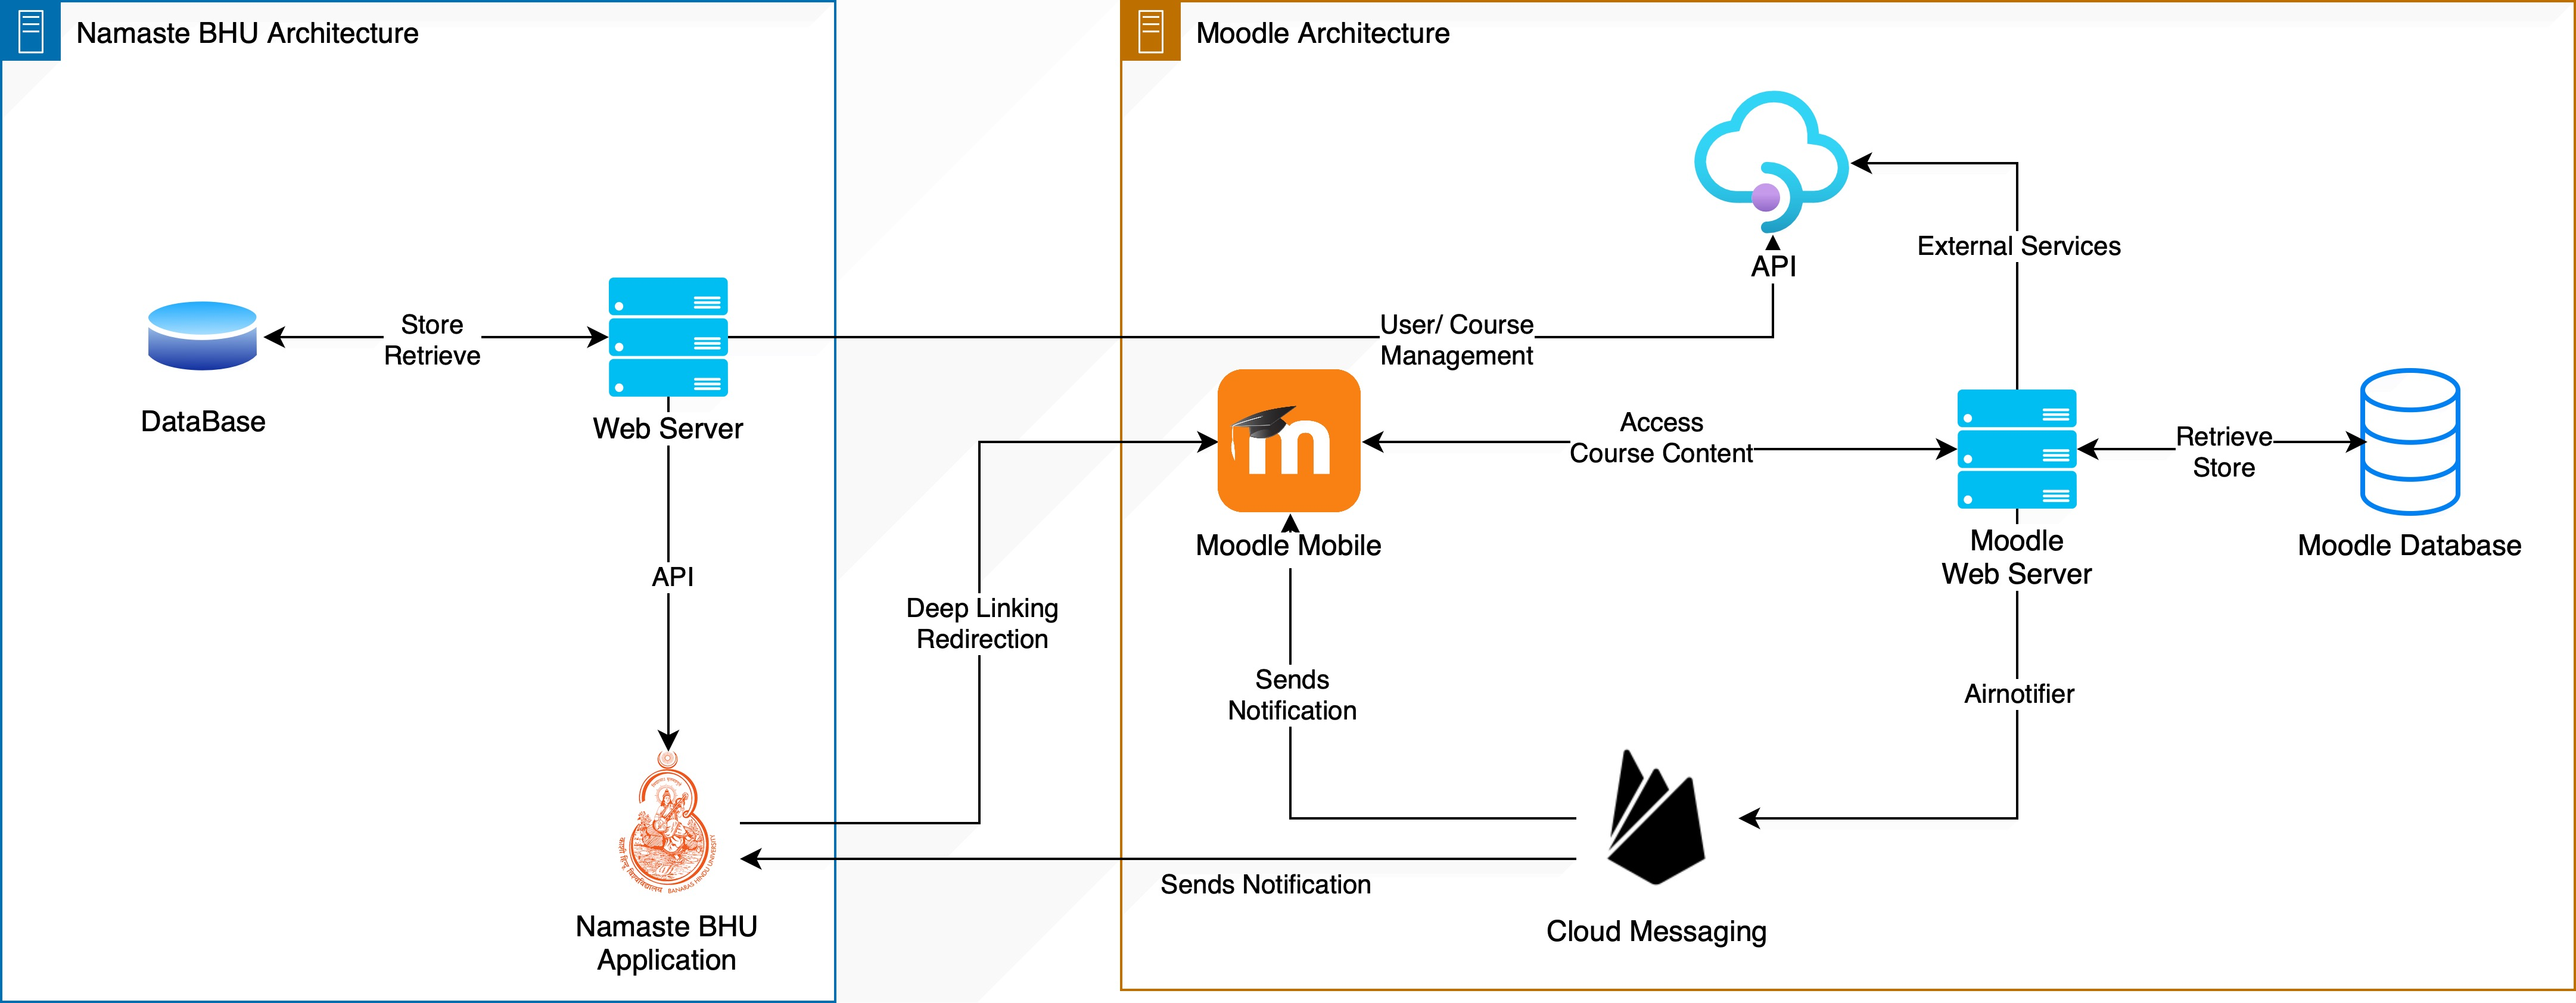
\includegraphics[width=\linewidth]{assets/img/proposed-arch.jpg}
    \caption{Proposed Architecture}
    \label{fig:proposed-arch}
\end{figure}

\textbf{Namaste Database Configuration}\\
The Namaste BHU database is configured to incorporate identifiers for courses, users, and access tokens required for seamless integration with Moodle. This involves updating the database schema to include fields for course IDs, user IDs, and authentication tokens, which facilitate the exchange of data between Namaste BHU and Moodle through APIs.

\textbf{Integration with Moodle APIs}\\
Moodle's APIs are utilized to establish communication between Namaste BHU and Moodle, enabling the exchange of data and functionalities between the two systems. Namaste BHU interacts with Moodle's APIs to retrieve course information, enroll users, synchronize content, and authenticate users seamlessly across both platforms.\\

\textbf{Moodle Web and Mobile Applications}\\
Users access Moodle's web and mobile applications to engage with course materials, activities, and resources offered through the integrated platform. Moodle's web application provides a comprehensive interface for accessing courses, participating in activities, and interacting with instructors and peers. The Moodle Mobile application extends the accessibility of Moodle to mobile devices, allowing users to learn on the go and stay connected with their academic progress.

\textbf{Seamless User Experience}\\
The proposed architecture aims to deliver a seamless user experience by integrating Namaste BHU's features and functionalities with Moodle's course management capabilities. Users can access course materials, receive notifications, participate in discussions, submit assignments, and view grades seamlessly across both platforms, enhancing their overall academic experience at Banaras Hindu University.

\clearpage
\chapter{IMPLEMENTATION}

\section{Overview}
The implementation process for integrating Moodle with the Namaste BHU application involves several key steps, including Moodle deployment, configuration of Moodle web server and mobile applications, installation of essential plugins, and seamless integration using Namaste BHU as a proxy. This overview outlines the main components and processes involved in the implementation that will be discussed in detail later.

The implementation begins with the deployment of Moodle, the open-source learning management system, on dedicated servers or cloud-based infrastructure. Moodle is installed and configured to provide a secure and reliable platform for hosting courses, managing users, and delivering educational content.

Several essential plugins are installed and configured within Moodle to enhance its functionality and integration capabilities.

The Namaste BHU application serves as a proxy for seamless integration between Namaste BHU and Moodle, enabling one-click login or single sign-on (SSO) functionality for users. Users can access Moodle content and functionalities directly from the Namaste BHU application without the need for separate authentication, streamlining the user experience and promoting engagement with the integrated platform.

\section{Moodle Deployment}
The deployment and configuration of Moodle on an Azure instance, along with the setup of the Moodle web server and mobile application, lay the groundwork for integrating Moodle with the Namaste BHU application.

Steps involved in Moodle Deployment on an instance:
\begin{enumerate}
    \item Create a new virtual machine (VM) instance on Azure
    \item Configure the VM with the necessary resources (CPU, memory, storage) and firewall rules (http 80 \& https 443).
    \item Install and configure the Apache web server, PHP, and MySQL database on the VM.
    \item Download the latest version of Moodle from the \href{https://moodle.org}{official website}.
    \item Extract the Moodle package into the web server directory.
    \item Configure the Moodle installation by providing database connection details, site settings, and administrator credentials.
    \item Run the Moodle installation script to complete the setup process.
    \item Verify that Moodle is accessible through the VM's public IP address or domain name.
    \item Configure a cron job to automate tasks such as scheduled tasks, background processing, and data maintenance within Moodle.
\end{enumerate}

\subsection{Web Server}
Moodle web server is the component responsible for hosting and serving Moodle's web-based interface to users. It provides access to courses, resources, activities, and communication tools within the Moodle environment.

\subsubsection*{Configuration}

\textbf{Appearence}\\
Customize the appearance of Moodle to align with the branding and identity of Namaste BHU. Modify themes, colors, logos, and fonts to create a cohesive user experience.

\begin{figure}[H]
    \centering
    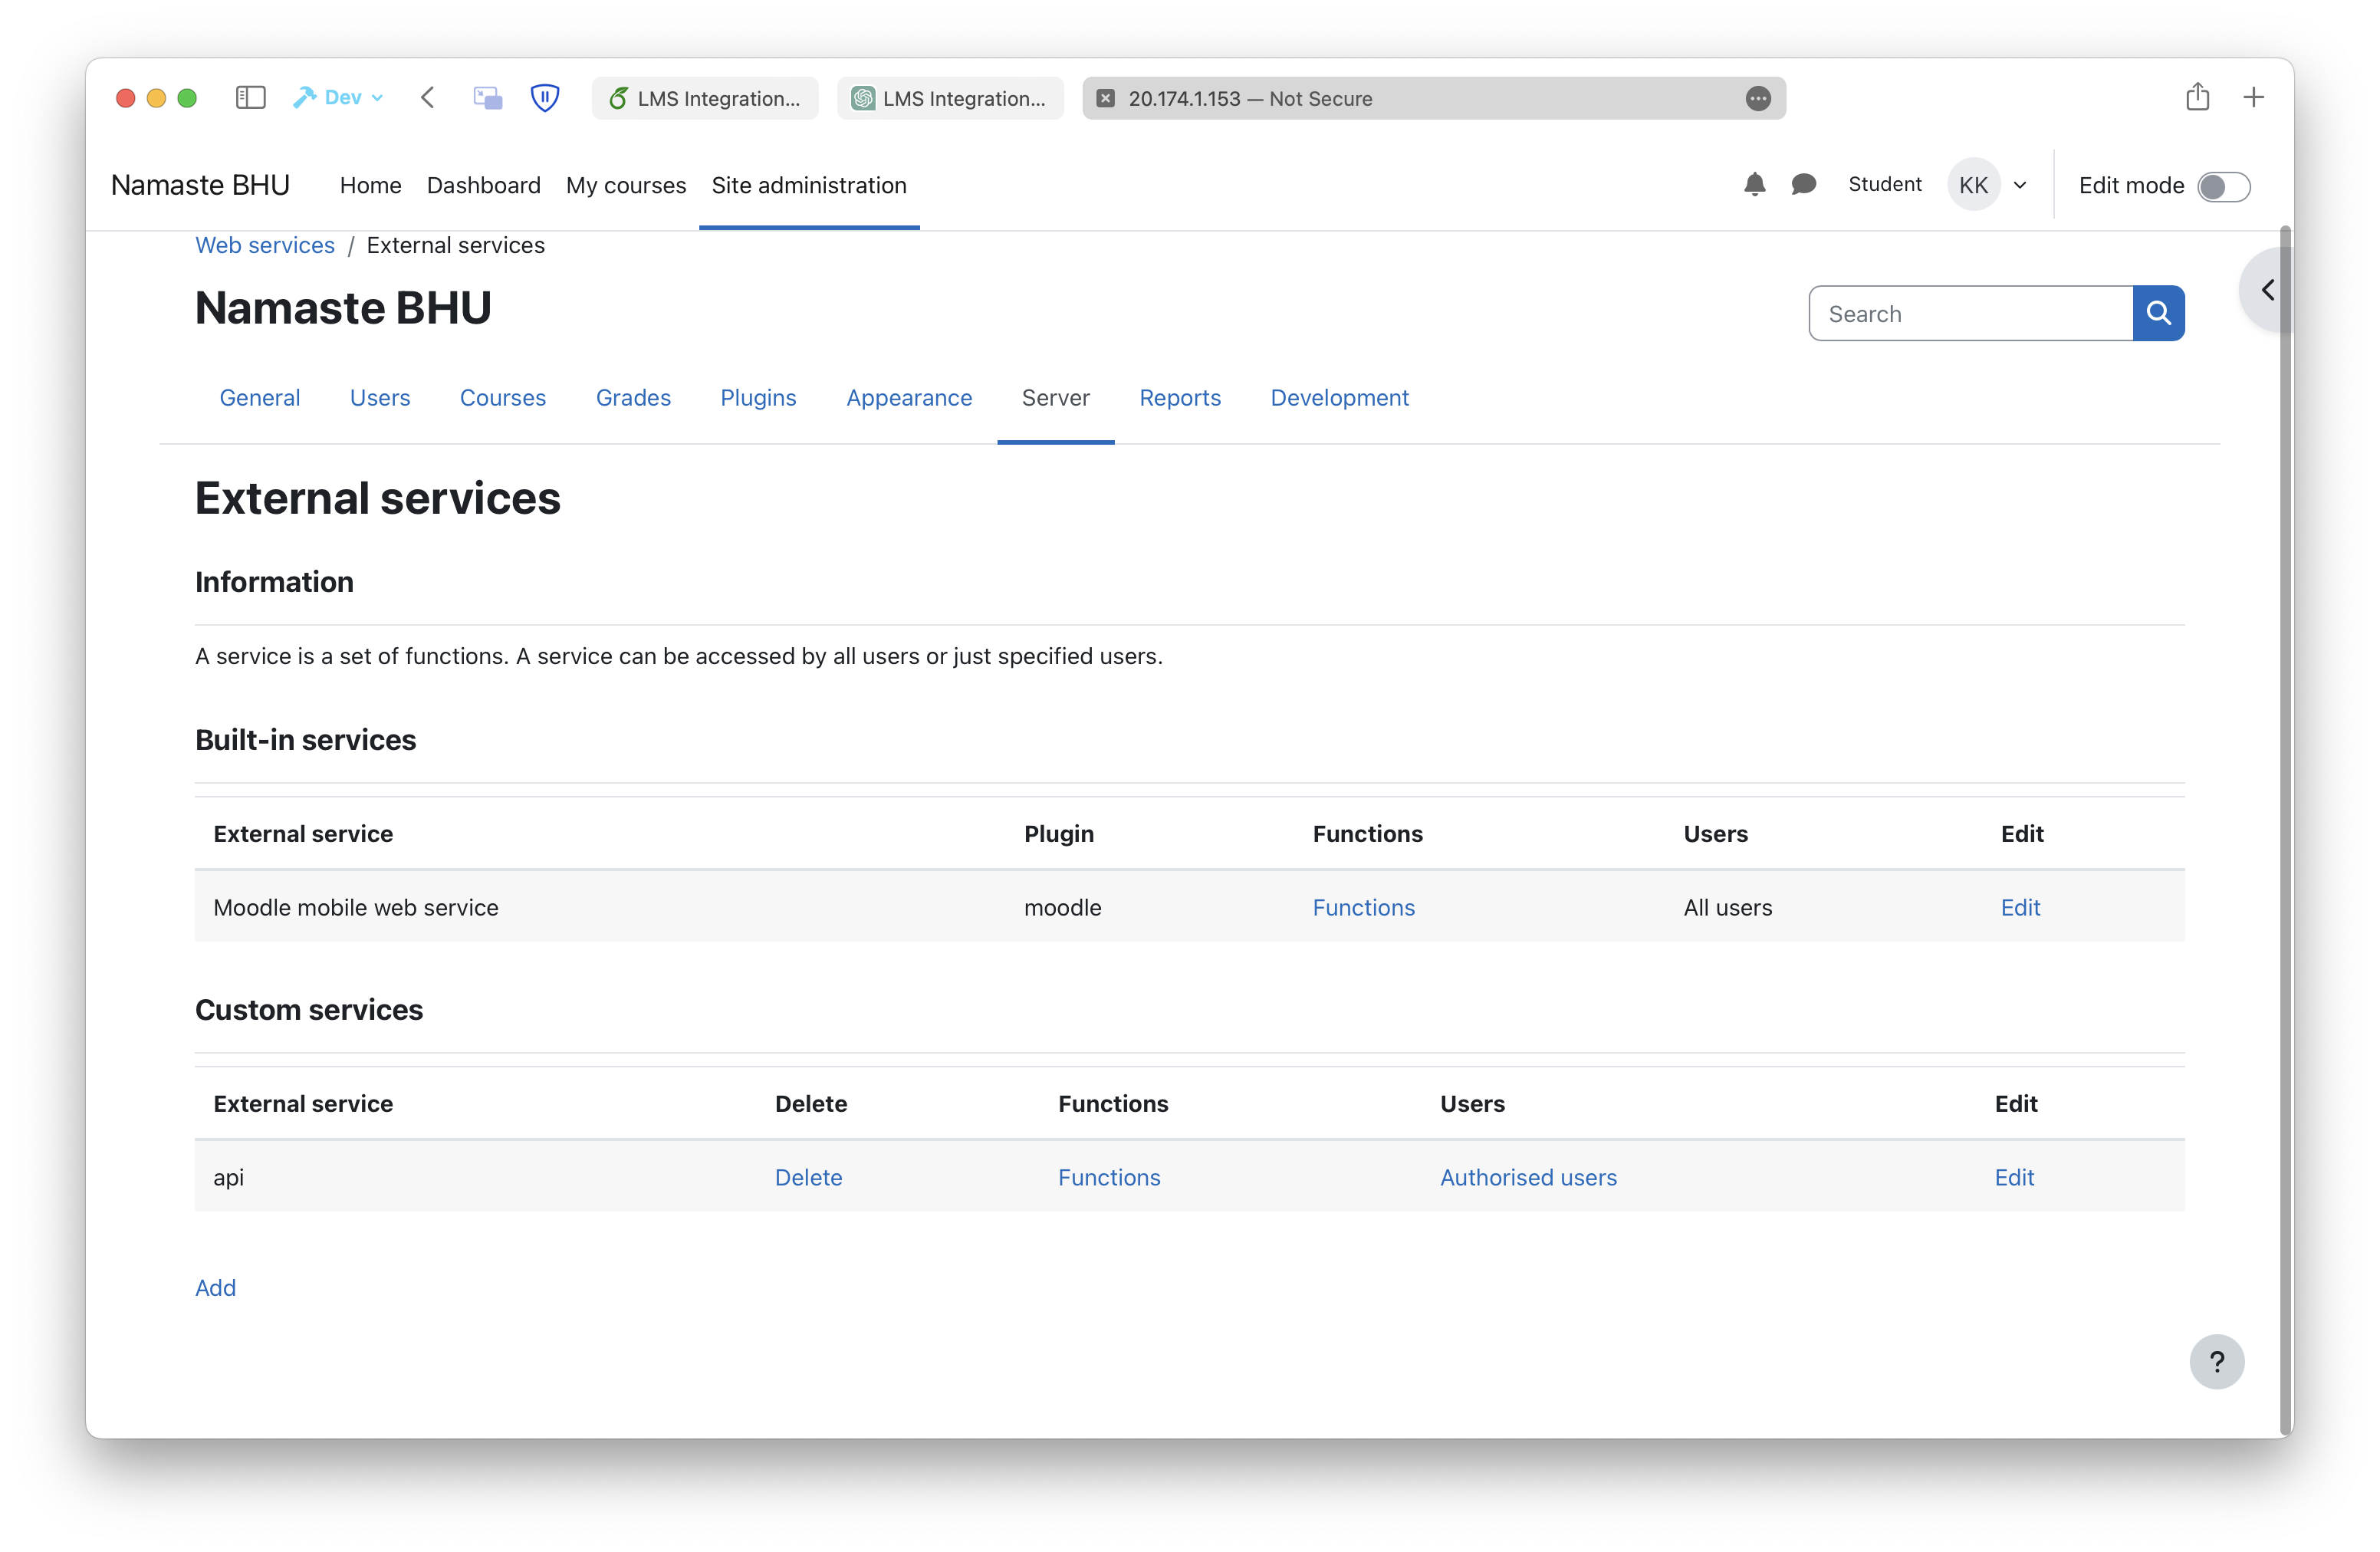
\includegraphics[width=0.75\linewidth]{assets/img/external-services.png}
    \caption{External Services}
    \label{fig:external-services}
\end{figure}

\textbf{Web Services}\\
Enable and configure web services to facilitate communication between Moodle and external systems, including Namaste BHU as show in Figure \ref{fig:external-services}. Define API endpoints, access permissions and the functionality to allow integration with external applications such as Namaste BHU.

\textbf{User Registration \& Login}\\
User registration options are configured to allow users to register manually or self-register for Moodle accounts, providing flexibility and convenience in onboarding new users and managing user accounts within the platform. Enabling login methods to provide users with options for authentication such as Manual Login and SSO from Namaste BHU.

\begin{figure}[h]
    \centering
    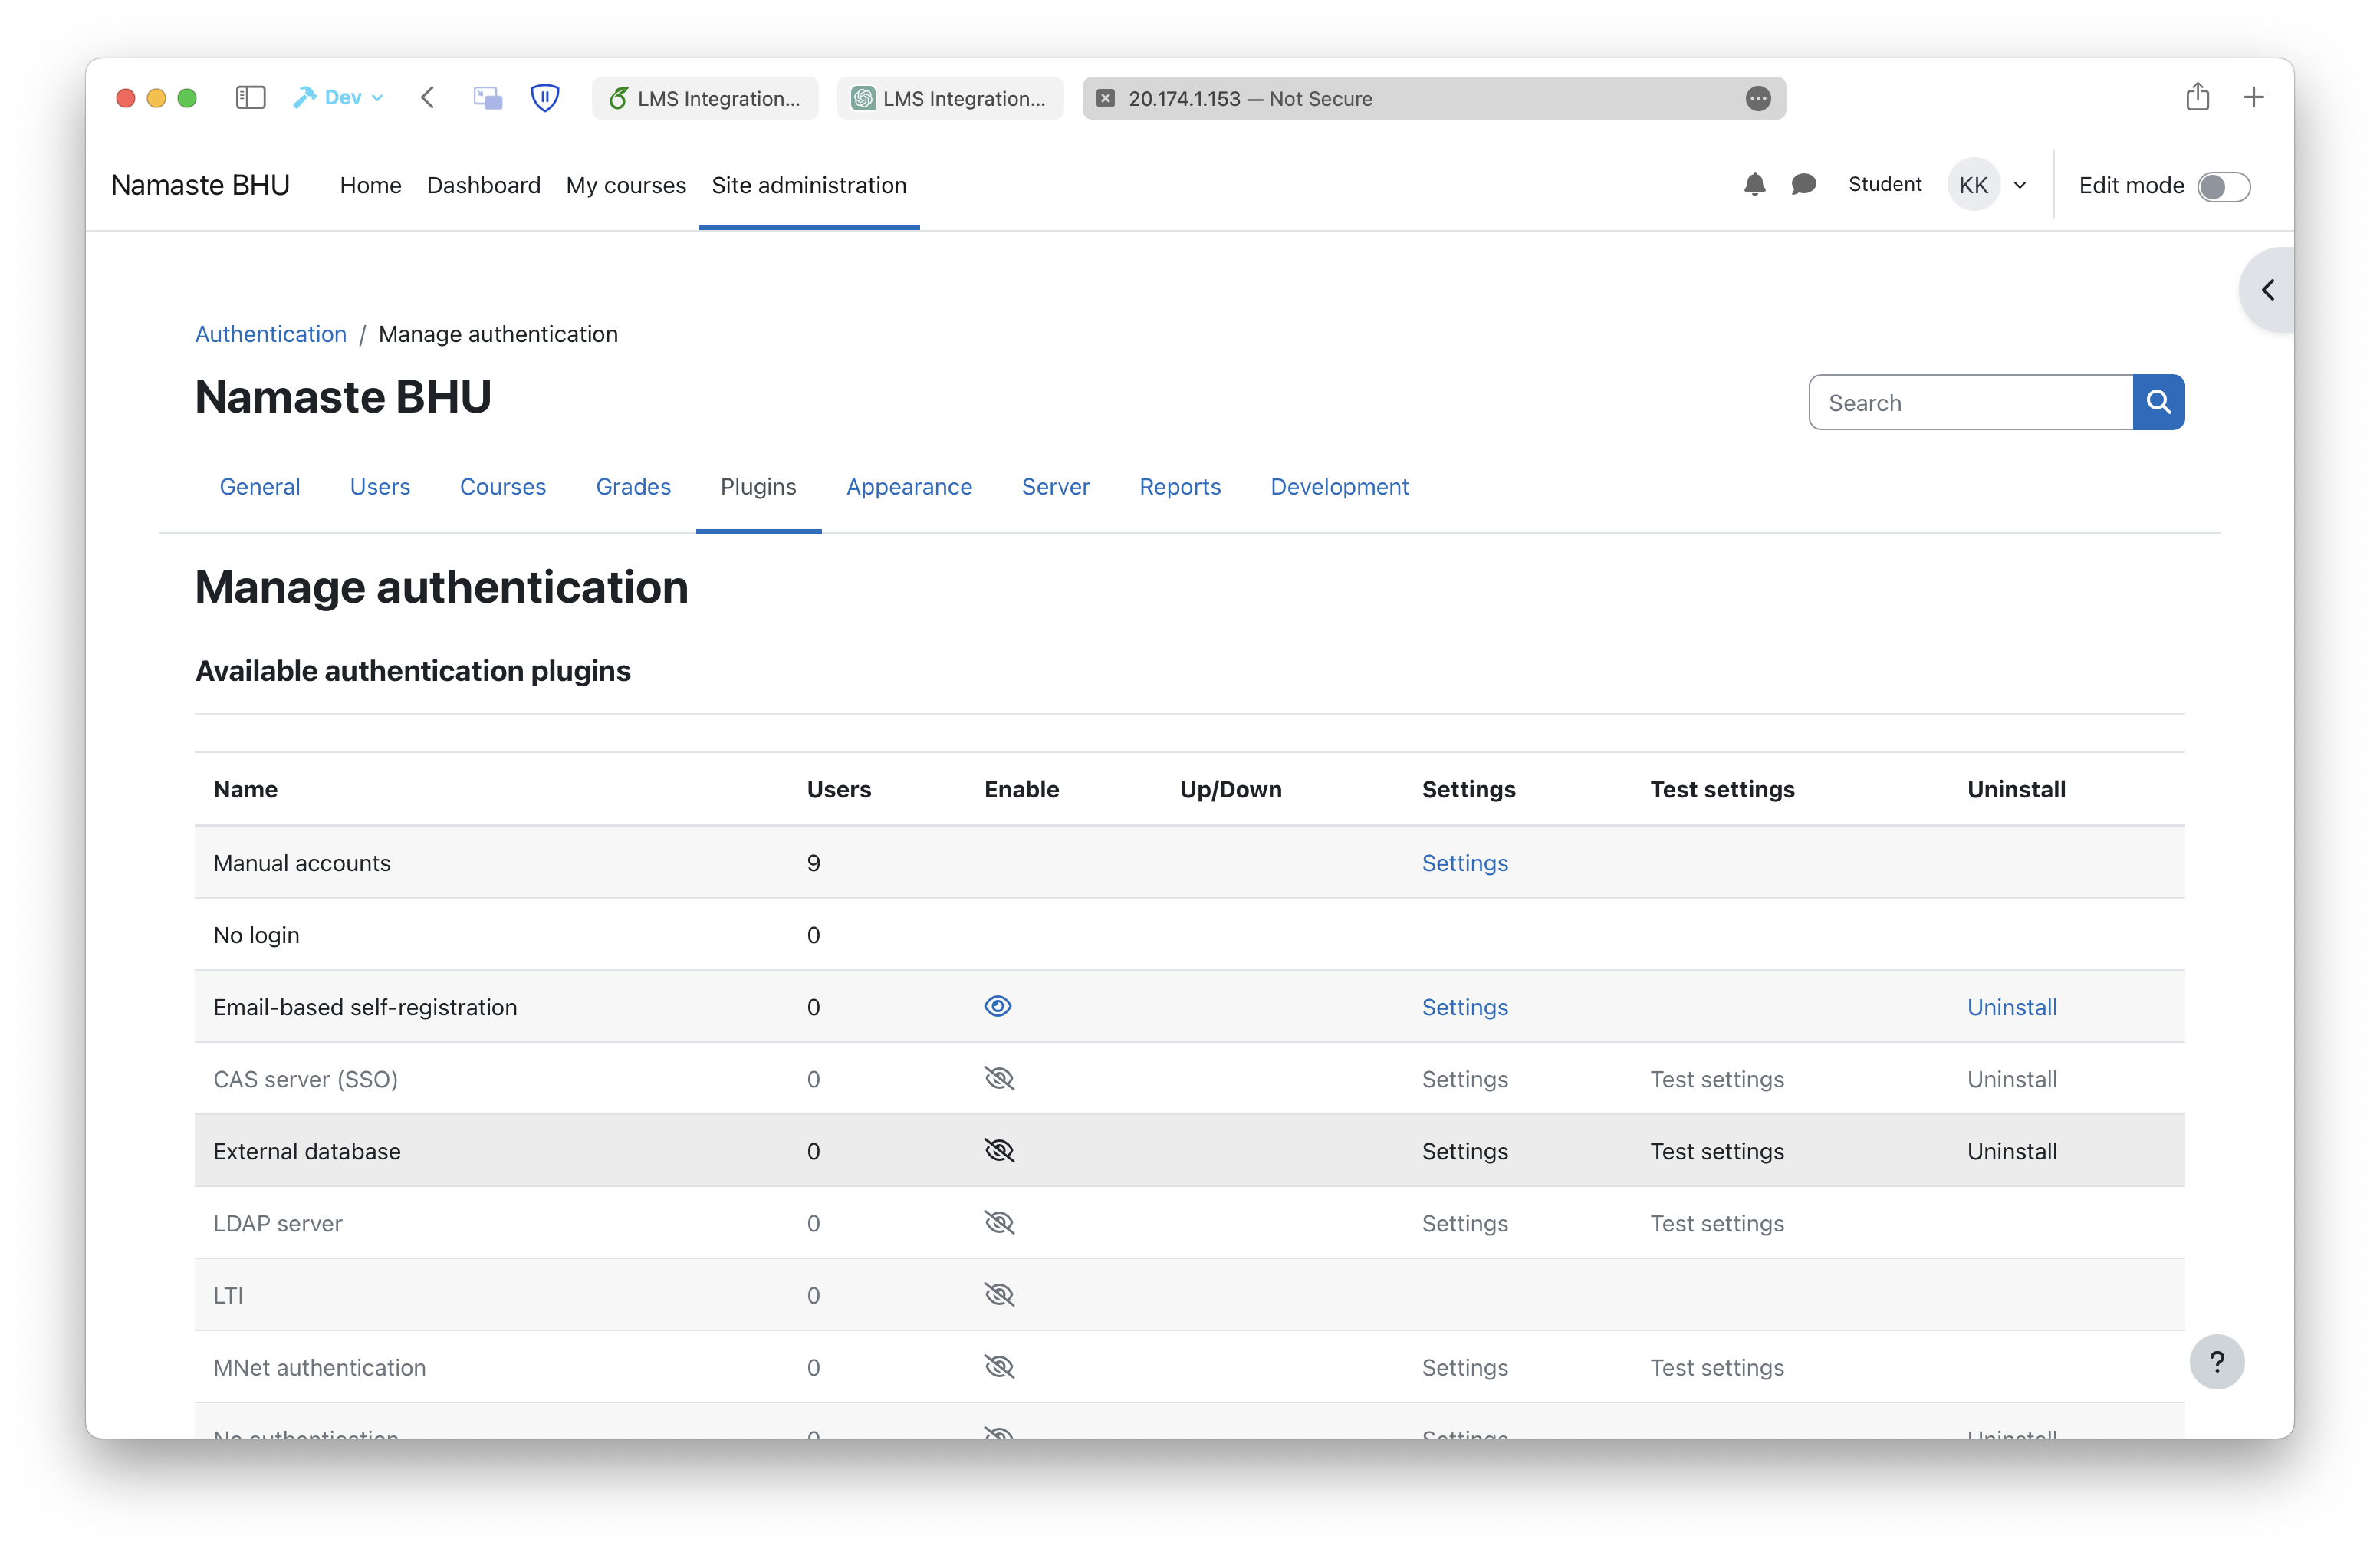
\includegraphics[width=0.75\linewidth]{assets/img/auth.png}
    \caption{Authentication}
    \label{fig:auth}
\end{figure}

\subsubsection*{Interface}

\textbf{Courses}\\
Moodle's course interface provides a centralized hub for accessing course materials, activities, resources, and communication tools, organized into categories and sections based on academic departments, programs, or topics.

\begin{figure}[H]
    \centering
    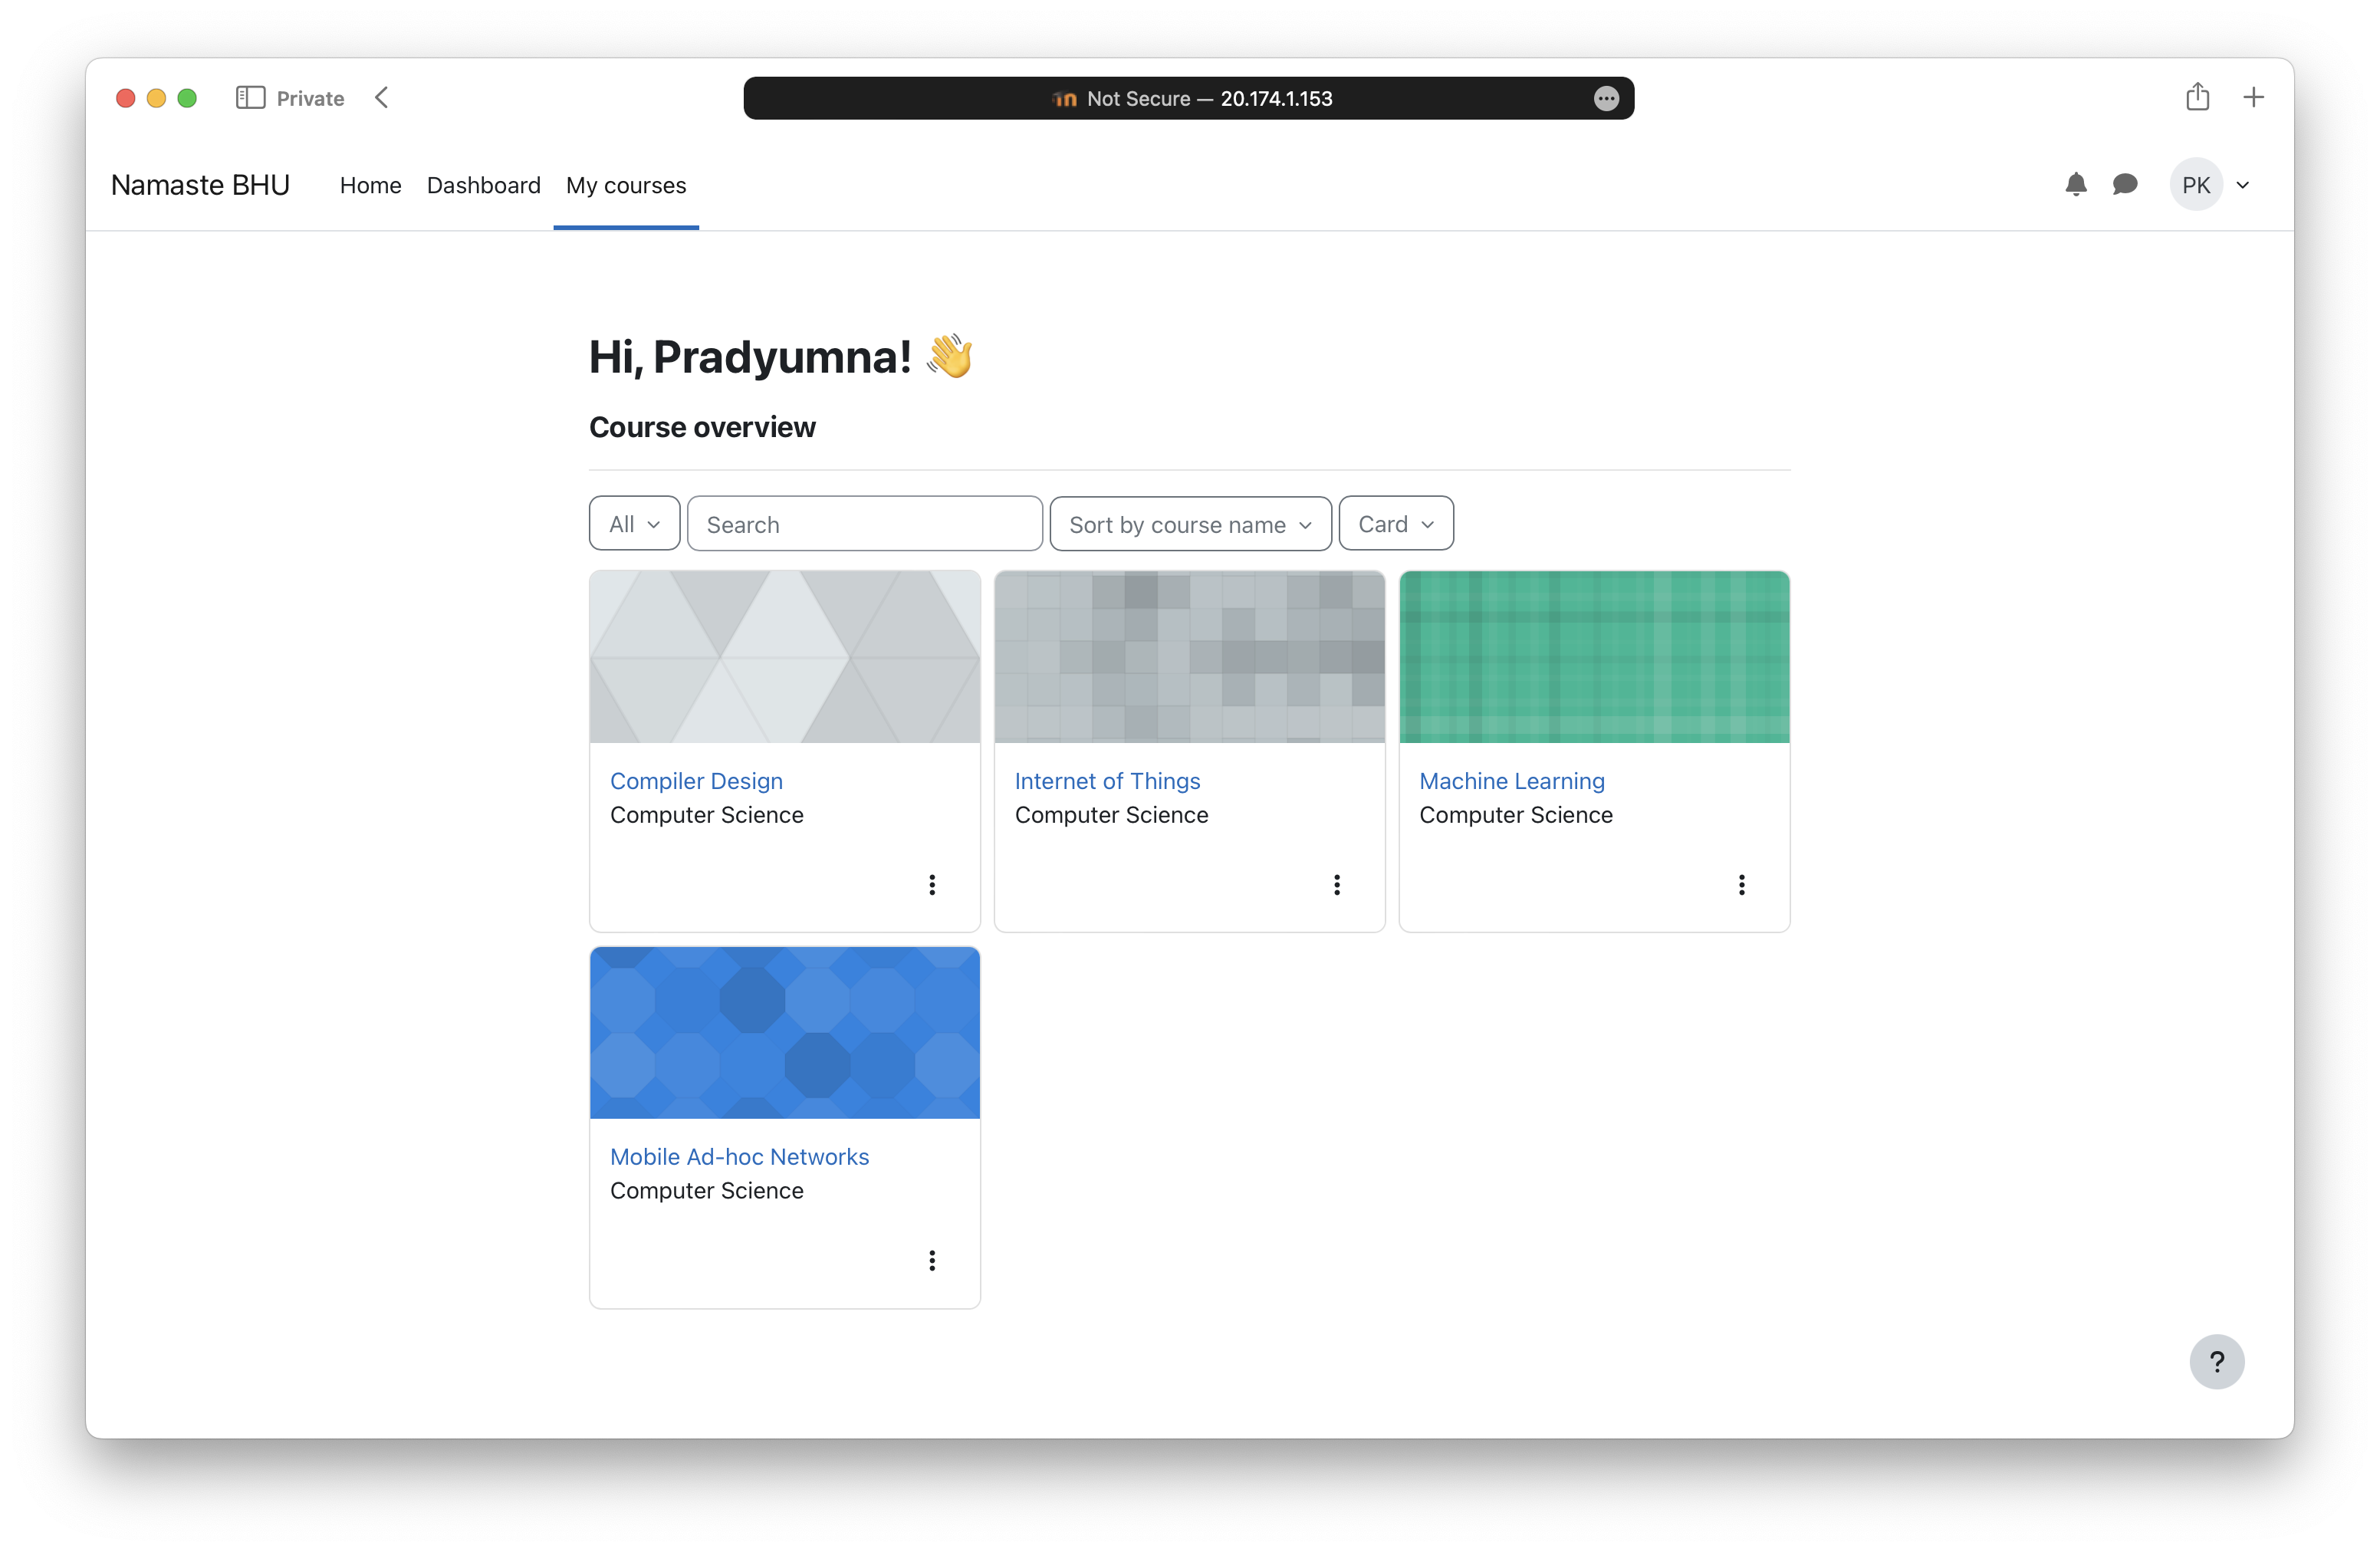
\includegraphics[width=0.75\linewidth]{assets/img/courses.png}
    \caption{Courses}
    \label{fig:courses}
\end{figure}

\textbf{Profile}\\
Users' profiles contain personalized information, preferences, and activity logs, allowing users to manage their accounts, view course enrollments, track progress, and communicate with instructors and peers.

\begin{figure}[h]
    \centering
    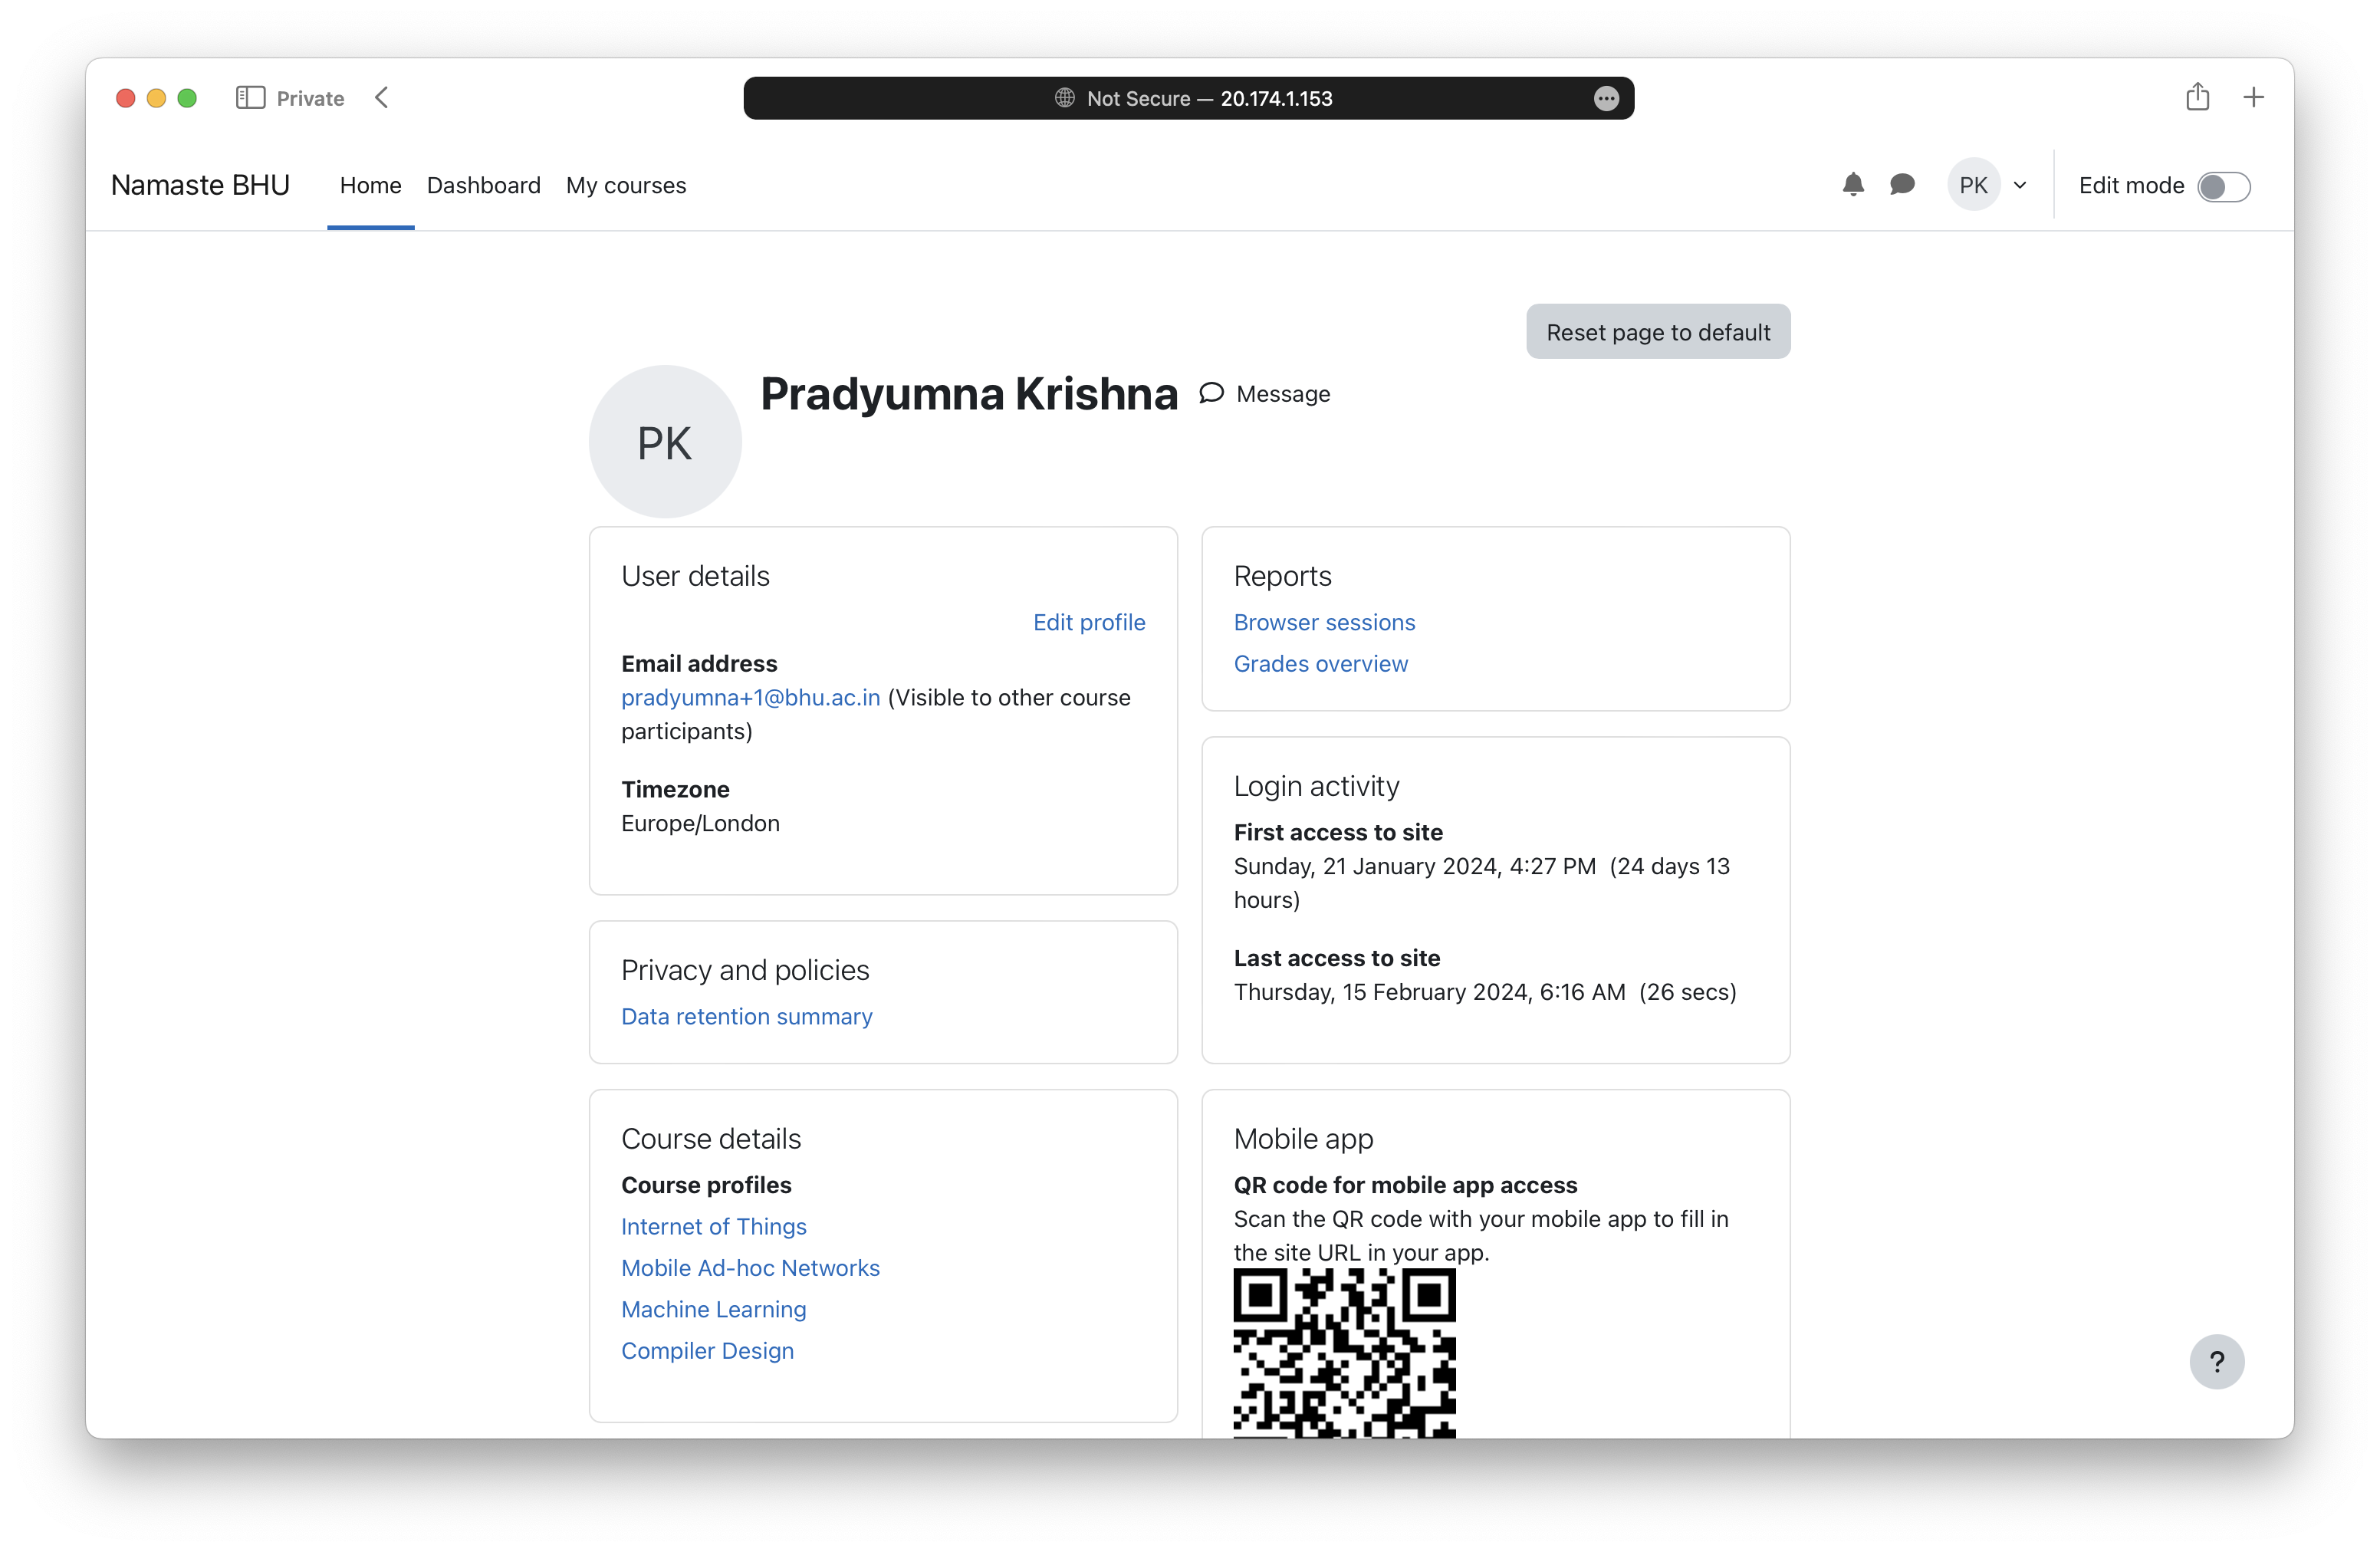
\includegraphics[width=0.75\linewidth]{assets/img/profile.png}
    \caption{Profile}
    \label{fig:profile}
\end{figure}

\subsection{Moodle Mobile}

Moodle Mobile extends the functionality of Moodle to mobile devices, providing users with access to course materials, activities, and communication tools on the go. Here's how the mobile application is enabled and configured:

\textbf{Enabling Mobile Application}\\
Enable the mobile app service in Moodle's administration settings to allow users to access Moodle through the mobile application. Configure mobile app settings, including site name, site URL, and authentication methods, to ensure compatibility and security.

\textbf{Logging through Mobile Application}\\
Users can log in to Moodle through the mobile application using their credentials from Namaste BHU or Moodle. Configure authentication settings to support seamless login and authentication, leveraging single sign-on (SSO) functionality if available.

\begin{figure}[h]
    \centering
    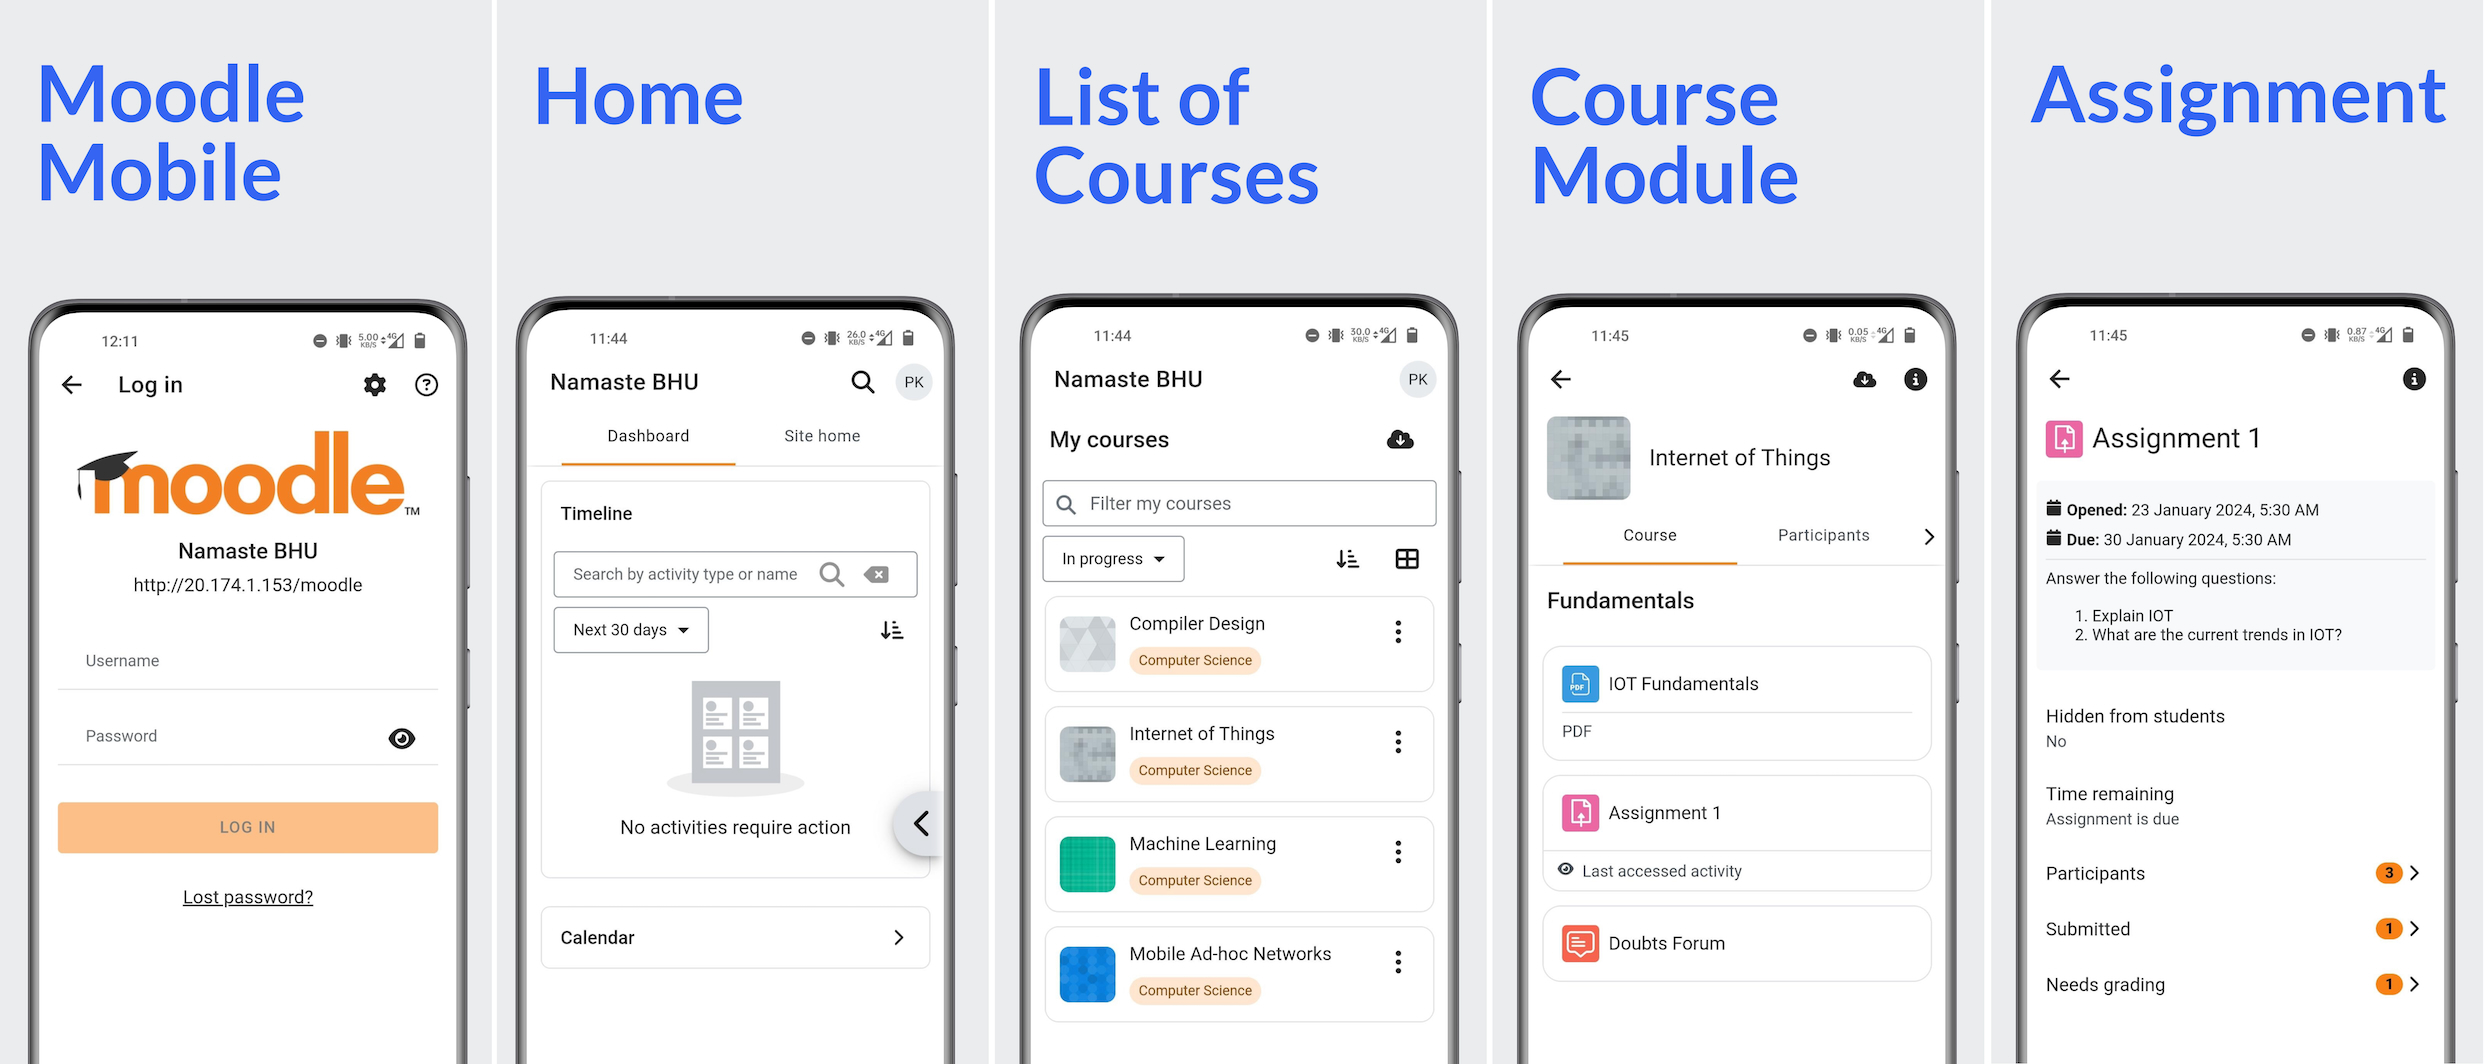
\includegraphics[width=\linewidth]{assets/img/moodle-mobile-opt.jpg}
    \caption{Moodle Mobile}
    \label{fig:moodle-mobile}
\end{figure}

\textbf{Interface and Navigation}\\
The Moodle Mobile application provides an intuitive interface and navigation experience for users, with features such as course listings, activity streams, notifications, messaging, and calendar integration. Users can easily navigate between courses, view course materials, participate in activities, and communicate with instructors and peers. The Moodle mobile interface is shown in Figure \ref{fig:moodle-mobile}.

\section{Plugins \& Extension}
These plugins and extensions enhance the functionality and capabilities of Moodle, enabling seamless integration with external systems, enhancing user experience, and extending the platform's capabilities.

\subsection{RESTful Protocol}

The \href{https://github.com/catalyst/moodle-webservice_restful}{RESTful Protocol} plugin was developed to address two main reasons: solving technical problems related to interfacing Moodle with services requiring unique URLs for each Moodle webservice call, and advancing the maturity of Moodle's webservice interface. Here are the key features of the RESTful Protocol plugin:

\begin{itemize}
    \item \textbf{Webservice Function as URL (Slash Parameter):} Instead of being passed as a query parameter, webservice functions are included in the URL. This allows each webservice to have a unique URL endpoint, enhancing accessibility and manageability.
    \item \textbf{Webservice Authorization Token as HTTP Header:} Authorisation tokens are passed using the 'Authorization' HTTP Header, ensuring secure communication between Moodle and external services.
    \item \textbf{Moodle Response Format as HTTP Header:} The desired Moodle response format is passed using the 'Accept' HTTP Header, providing flexibility in specifying the format of the response data.
\end{itemize}


A sample API call to fetch courses using RESTful Protocol:
\begin{minted}[breaklines=true]{http}
POST /moodle/webservice/restful/server.php/core_course_get_courses HTTP/1.1
Host: localhost
Authorization: <token>
Content-Type: application/json
Accept: application/json
[
    { 
        "id": "2",
        "shortname": "IOT",
    }
]
\end{minted}

\subsection{Auth UserKey}
The \href{https://moodle.org/plugins/auth_userkey}{Auth UserKey} plugin facilitates simple one-way Single Sign-On (SSO) between Moodle and external web applications. It allows users to log in to Moodle without typing their username and password by generating one-time login URLs. Here are the main features of the Auth Userkey plugin:

\begin{itemize}
    \item \textbf{Web Call to Moodle}: External applications make a web call to Moodle and provide a matching field to find the required user and generate a one-time login URL.
    \item \textbf{Simple Integration}: The plugin simplifies the integration process between Moodle and external web applications, enhancing user experience and streamlining the authentication process.
\end{itemize}

This enables an endpoint for user login:
\begin{minted}[breaklines=true]{http}
GET /auth/userkey/login.php?key={token} HTTP/1.1
HOST: localhost
\end{minted}

\subsection{Airnotifier}
\href{https://github.com/dcai/airnotifier}{AirNotifier} is a user-friendly and powerful application server for sending real-time notifications to mobile and desktop applications. It provides a unified web service interface to deliver messages to multiple devices using multiple protocols.

\section{Seamless Integration}
\subsection{Flow}

The basic workflow of the integration between Moodle and Namaste BHU involves the following steps:

\begin{figure}
    \centering
    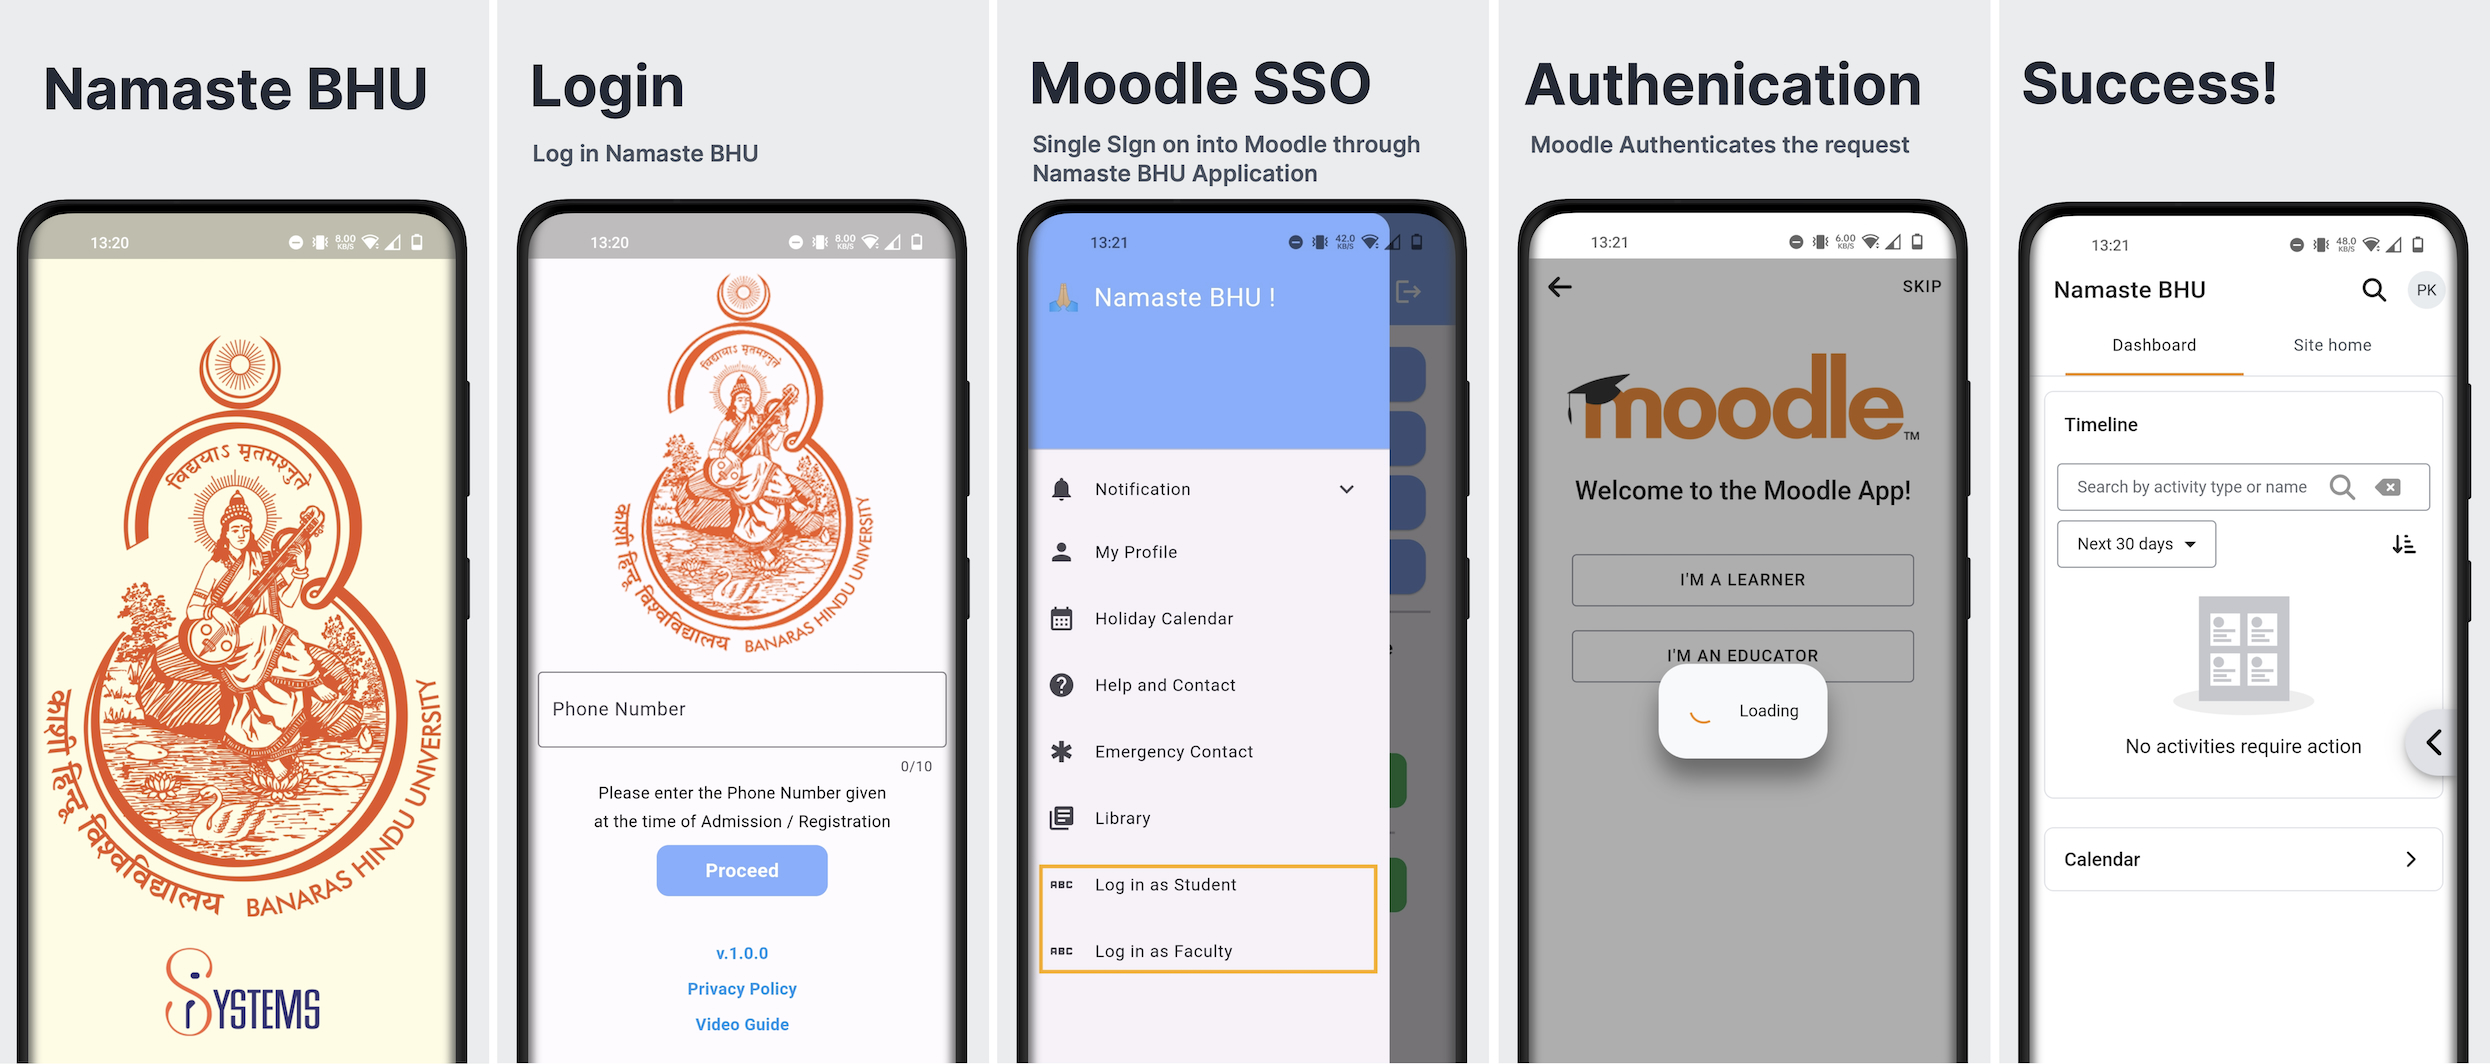
\includegraphics[width=\linewidth]{assets/img/flow-opt.jpg}
    \caption{Integration Flow}
    \label{fig:flow}
\end{figure}

\begin{enumerate}
    \item Users log in to the Namaste BHU application using their credentials.
    \item Upon successful authentication, Namaste BHU retrieves the list of courses associated with the user from its database.
    \item Namaste BHU prepares a redirection URL that includes the necessary parameters, such as the user ID, user token, redirect, and course ID.
    \item The user is redirected from Namaste BHU to Moodle through Deep Linking.
    \item Users are authenticated automatically within Moodle through token, eliminating the need for separate authentication.
    \item Upon redirection, the Moodle Mobile application accesses the course content and resources associated with the user's enrolled courses, providing seamless access to educational materials and activities.
\end{enumerate}

\subsection{Database Mapping}

Changes are required in the Namaste BHU database to facilitate seamless integration with Moodle. These changes include:

\begin{itemize}
    \item \textbf{UserID}: Namaste BHU database must store the Moodle user ID to establish a mapping between Namaste BHU users and Moodle users.
    \item \textbf{User Token}: A user token is generated and stored in the Namaste BHU database for authentication and authorization purposes when accessing Moodle resources.
    \item \textbf{Course ID}: Namaste BHU database must store the Moodle course ID to identify the courses in which users are enrolled.
\end{itemize}

These database mappings enable efficient data exchange and synchronization between Namaste BHU and Moodle, ensuring a seamless user experience.\\

\subsection{Deep Linking}
Deep linking enables users to navigate to a specific piece of content or perform a specific action within a mobile application, bypassing the app's home screen and providing a seamless user experience. It involves associating a URL with a particular location or function within the app, allowing users to access that content directly from an external source, such as a website, email, or another app.

\begin{figure}[h]
    \centering
    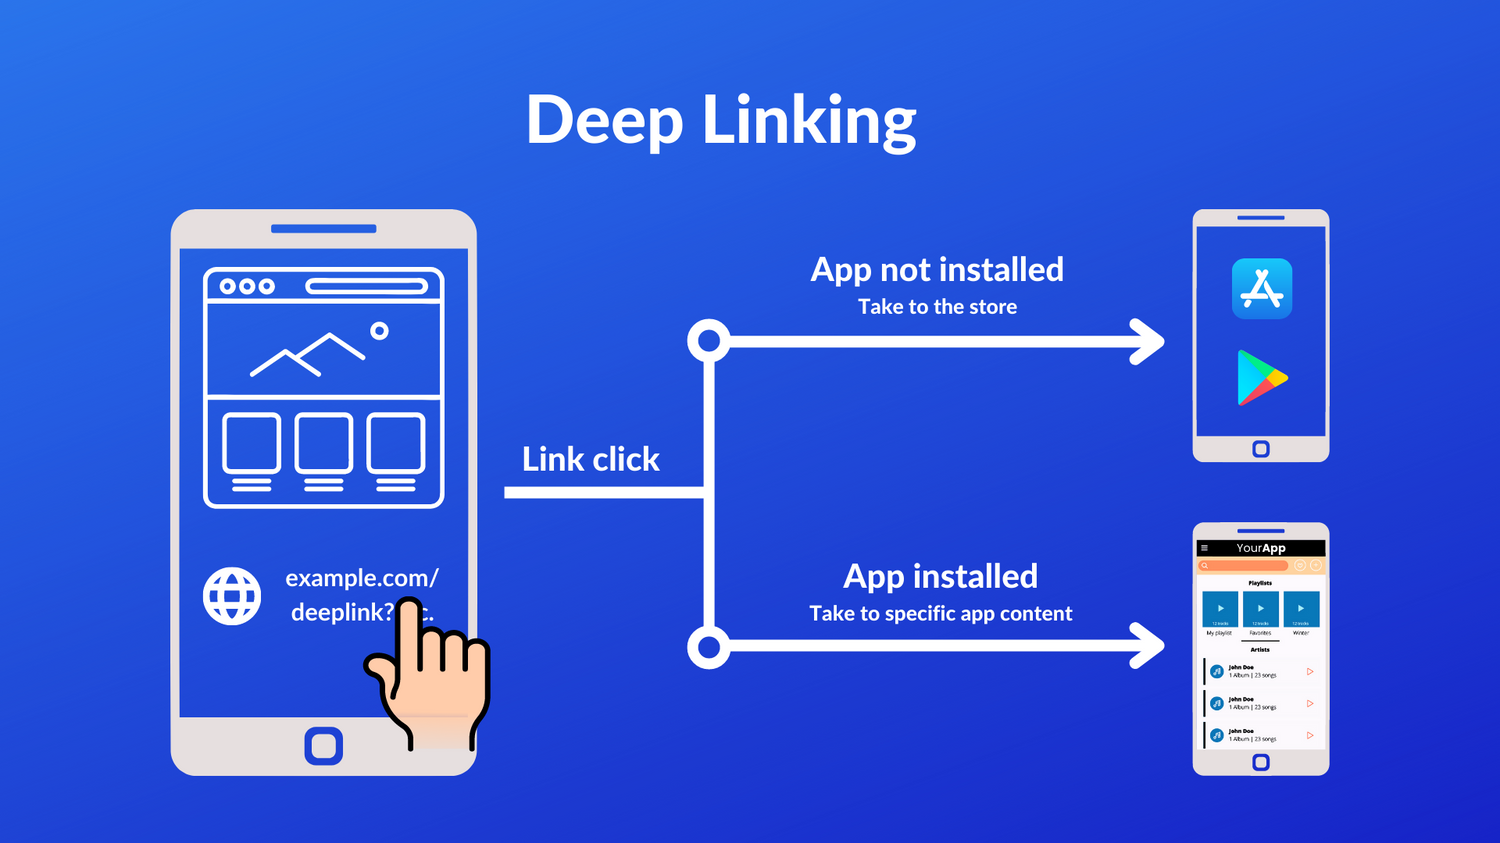
\includegraphics[width=0.75\linewidth]{assets/img/deeplinking.png}
    \caption{Deep Linking}
    \label{fig:deep-linking}
\end{figure}

\textbf{How Deep Linking Works}
\begin{itemize}
    \item Deep links typically have a specific URL structure that includes a scheme (e.g., "\texttt{https://}" or "\texttt{myapp://}"). Here, \texttt{moodlemobile://}.
    \item Mobile applications register deep links with the operating system to handle incoming link requests. This involves specifying the URL scheme and associated actions or destinations within the app.
    \item As shown in Figure \ref{fig:deep-linking} when a user clicks on a deep link, the operating system checks if the corresponding app (Moodle Mobile) is installed on the device. If the app is installed and registered to handle the deep link, the operating system opens the app and passes the link to it.
    \item The app receives the deep link and navigates the user to the specified location or performs the specified action within the app. This could involve displaying a specific screen, loading particular content, or executing a particular function.
\end{itemize}

The format to create the links for Moodle Mobile is the following:
\begin{minted}[breaklines=true]{text}
    moodlemobile://https://username@domain.com?token=TOKEN &redirect=http://domain.com/course/view.php?id=2
\end{minted}



\subsection{Messaging}
The Moodle Messaging workflow involves the generation of notifications within Moodle, communication with the AirNotifier service to deliver push notifications via Firebase Cloud Messaging, and user interaction with the notifications on their devices. This seamless process ensures timely delivery of important updates, announcements, and events to users within the Moodle and Namaste BHU ecosystems, enhancing communication and engagement within the academic community.

\begin{figure}
    \centering
    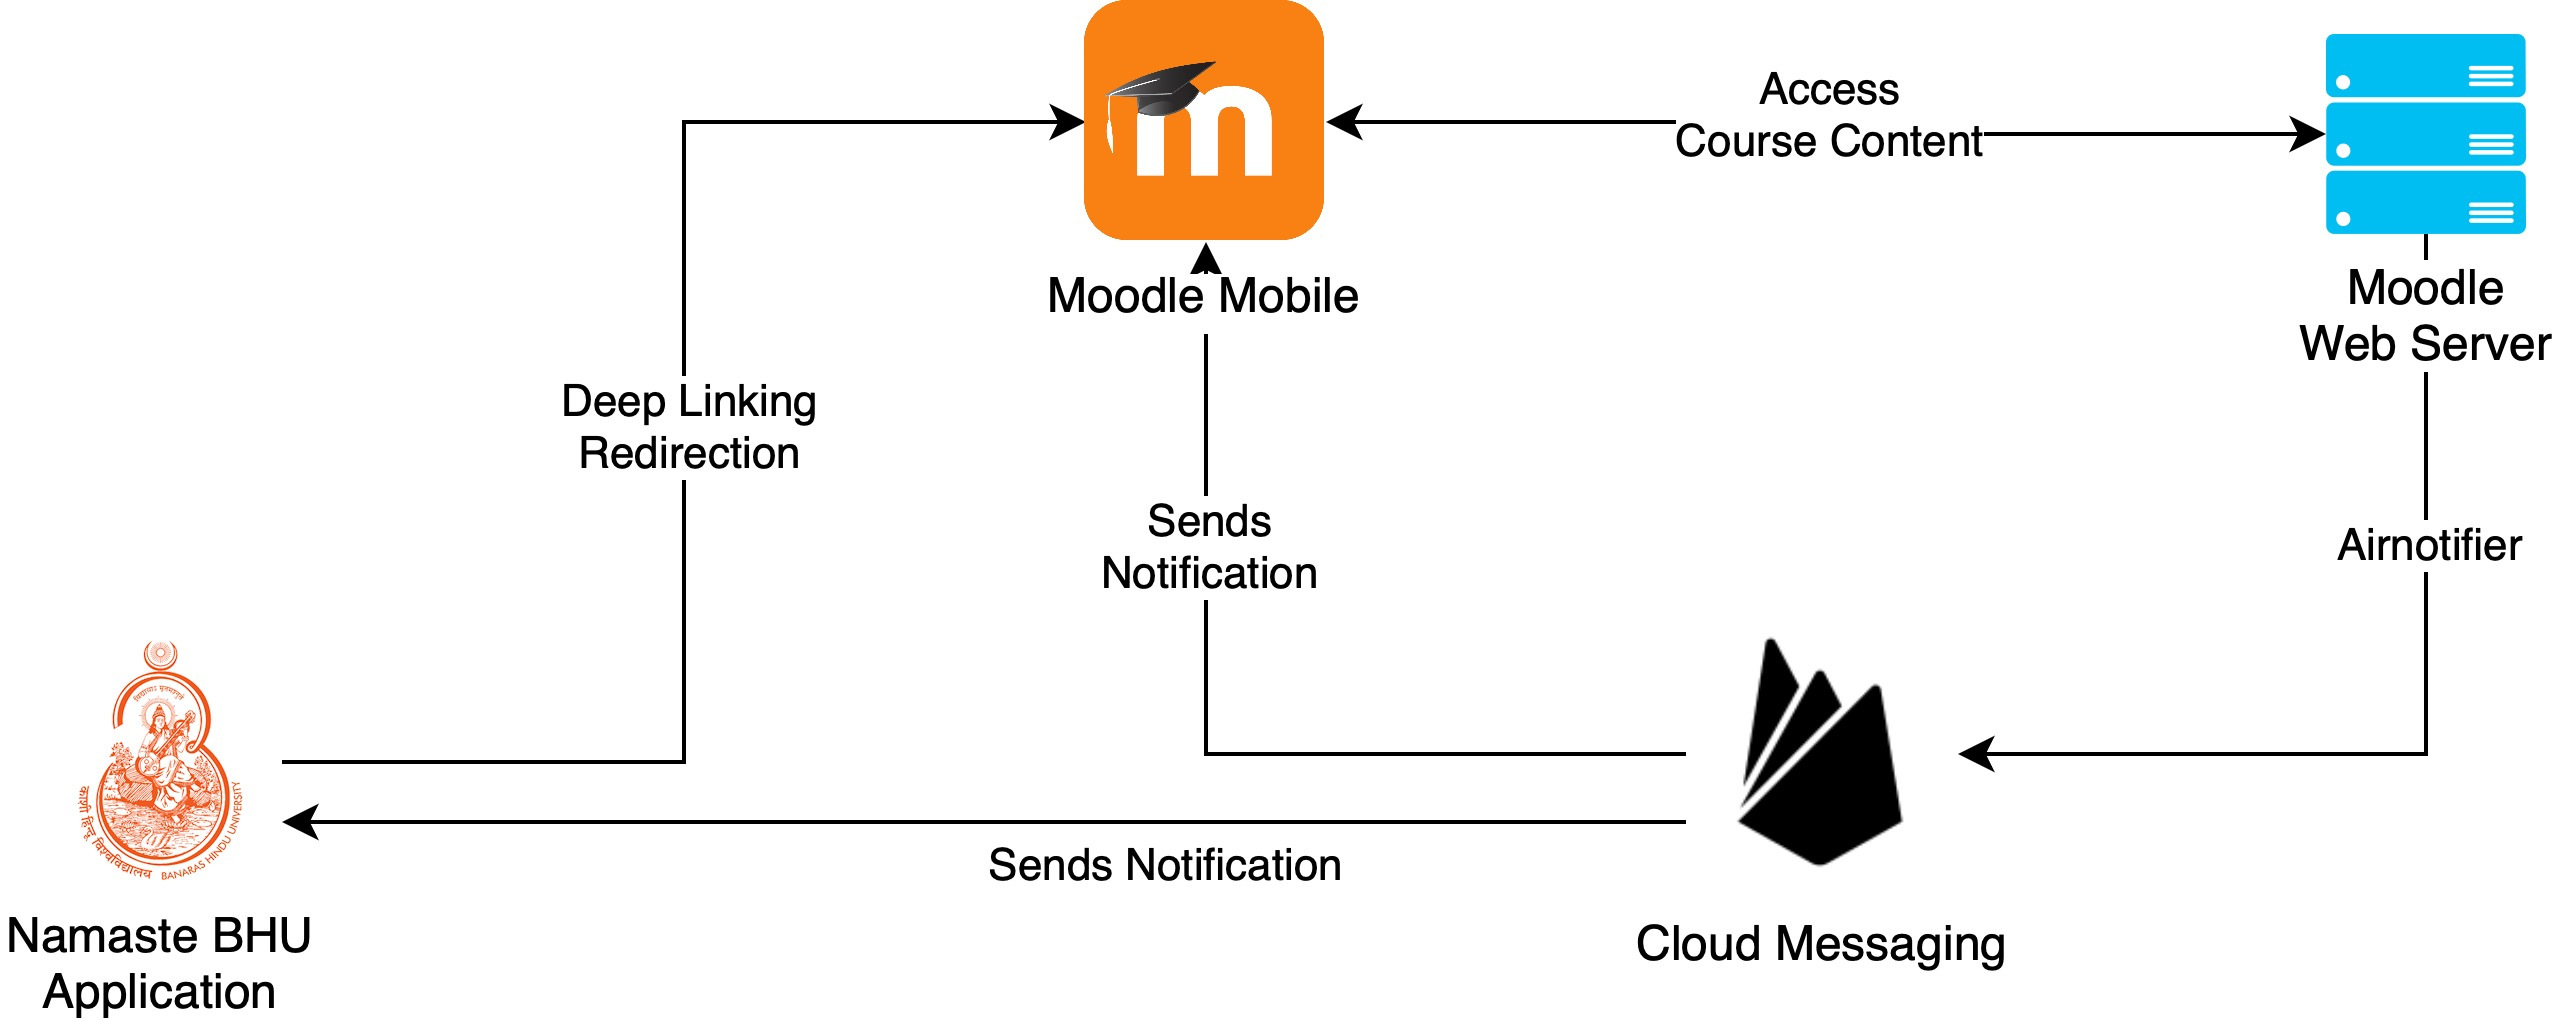
\includegraphics[width=0.75\linewidth]{assets/img/notification-flow.jpg}
    \caption{Notification Flow}
    \label{fig:notification-flow}
\end{figure}

\textbf{Workflow}\\
The Moodle platform detects a trigger event that warrants a notification, such as a new announcement, a course update, or an upcoming deadline.  Upon detecting the trigger event, Moodle generates a notification message containing relevant information, such as the event type, title, description, and associated course or user.

Moodle communicates with the AirNotifier service through its API, passing along the notification message and the device ID of the recipient. The device ID uniquely identifies the user's device and allows AirNotifier to deliver the notification to the correct recipient. 

AirNotifier utilizes Firebase Cloud Messaging (FCM) credentials to send push notifications to both Namaste BHU and Moodle Mobile applications. These credentials include the Firebase server key and project ID, which authenticate the sender and authorize the delivery of notifications through the FCM service.

Using the Firebase credentials, AirNotifier sends push notifications to the respective devices associated with the device ID provided by Moodle. The notification is delivered to the user's device through the FCM service, ensuring real-time delivery and visibility to the recipient.


\subsection{API Services}
API services are utilized for various purposes to manage both Namaste and Moodle servers, including:

\begin{itemize}
    \item \textbf{Course Management}: Creating, updating, and managing courses within Moodle through API calls from the Namaste BHU application.
    \item \textbf{User Management}: Creating, updating, and managing user accounts within Moodle through API calls from the Namaste BHU application.
    \item \textbf{Authentication}: Authenticating users and generating access tokens for accessing Moodle content through API calls from the Namaste BHU application.
    \item \textbf{Data Synchronization}: Synchronizing user data, course information, and other relevant data between Namaste BHU and Moodle databases through API services to ensure consistency and accuracy.
\end{itemize}

\clearpage
\chapter{RESULTS AND DISCUSSIONS}

The integration of Moodle with the Namaste BHU application represents a significant milestone in enhancing the academic experience and administrative efficiency at Banaras Hindu University. Through meticulous deployment, configuration, and integration efforts, the project has successfully established a seamless connection between the two platforms, enabling students, faculty, and staff to access course materials, communicate, and collaborate more effectively.

\textbf{Moodle}\\
The deployment of Moodle on the Azure cloud infrastructure, along with the installation of essential plugins and extensions, has provided a robust and scalable learning management system for managing courses, resources, and activities. Moodle incorporates key features and functionalities, such as RESTful Protocol, Auth Userkey, and AirNotifier, to enhance accessibility, security, and communication within the platform.

The moodle is hosted at \href{http://20.174.1.153/moodle}{\texttt{http://20.174.1.153/moodle}} on an Azure Instance.

\begin{figure}[h]
    \centering
    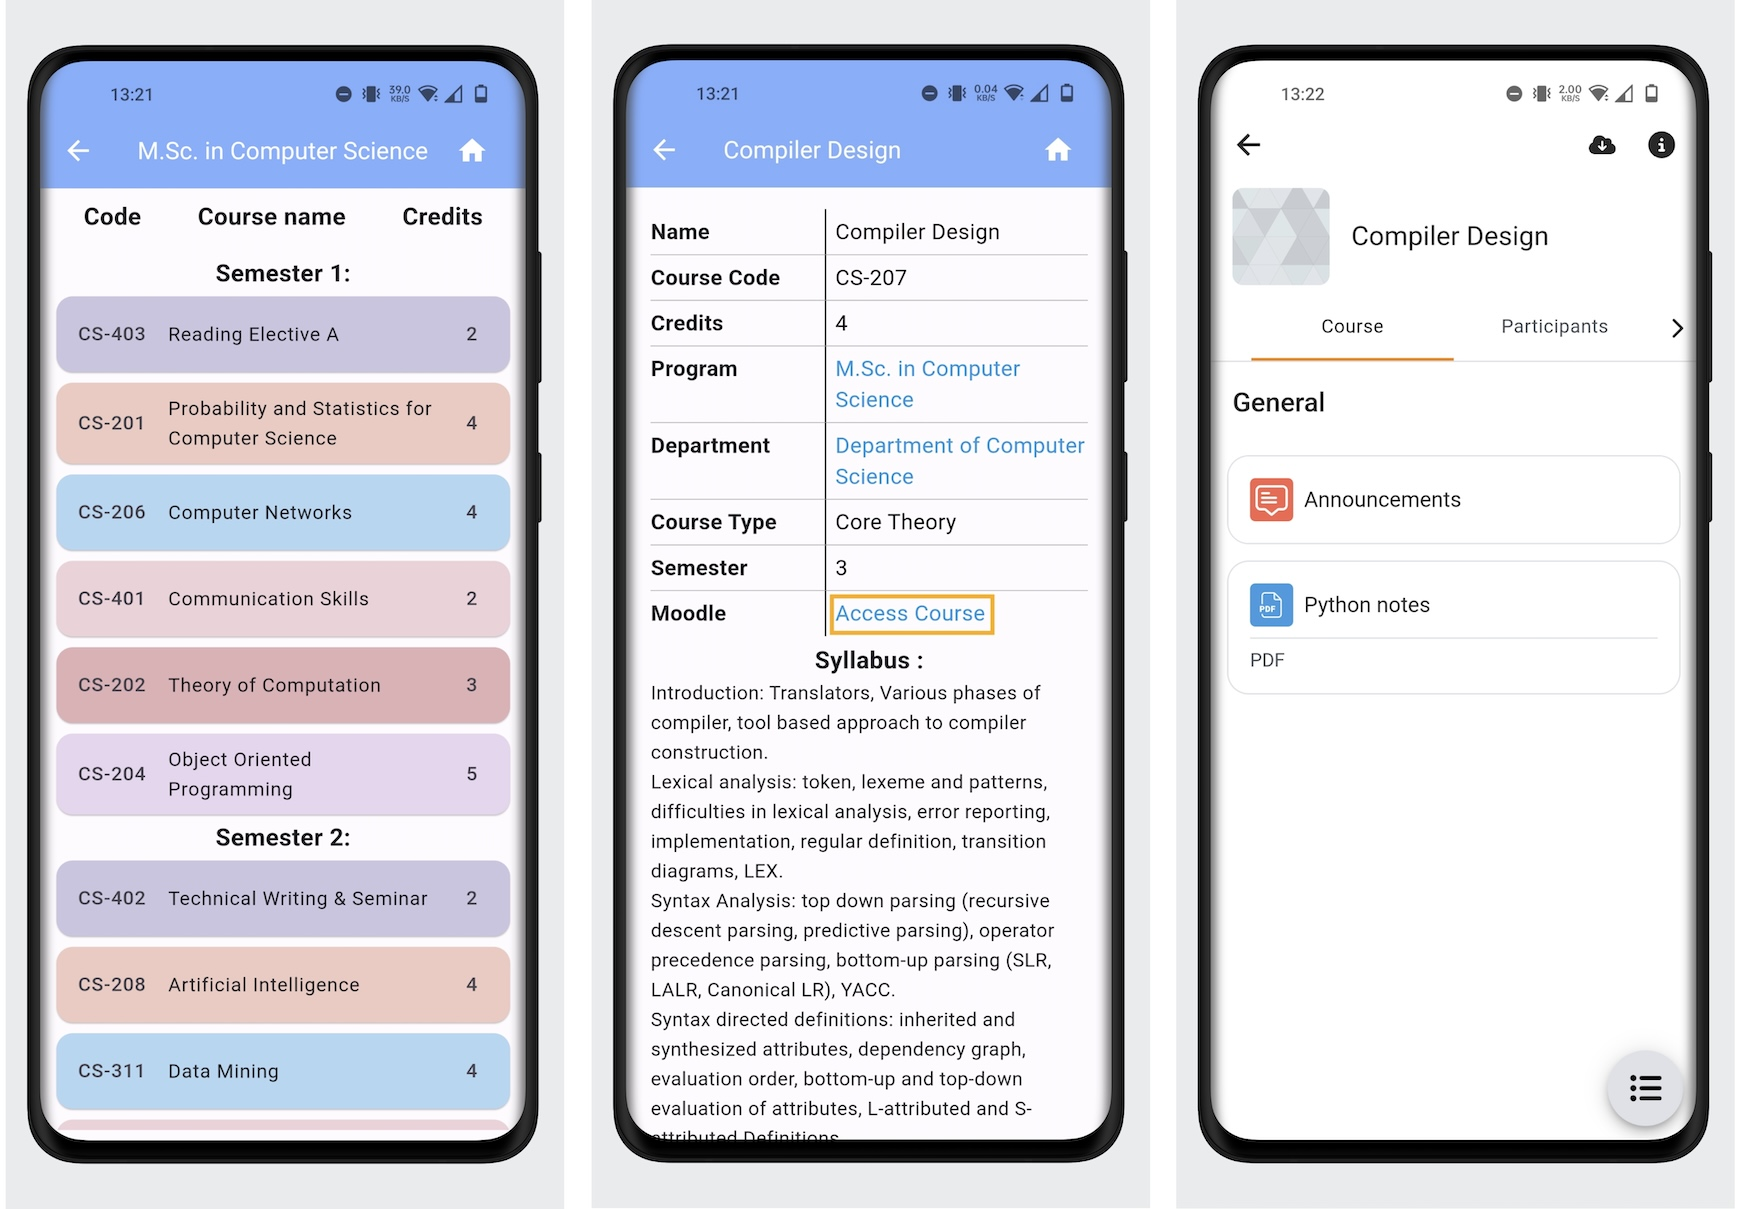
\includegraphics[width=\linewidth]{assets/img/result-opt.jpg}
    \caption{Final Application}
    \label{fig:result}
\end{figure}

\textbf{Namaste BHU}\\
The Namaste BHU Architecture underwent updates and enhancements to facilitate seamless integration with Moodle. New features and functionalities were introduced in Namaste BHU to support single sign-on (SSO) through deep linking of the Moodle Mobile App. The updated Namaste BHU application serves as a central hub for accessing Moodle content, enabling users to seamlessly navigate between the two platforms and engage with course materials, announcements, and discussions. In future it will also deliver notification from Moodle through Airnoitifier.

\clearpage
\chapter{CONCLUSION}
The integration of Moodle with the Namaste BHU application represents a significant achievement in enhancing the educational experience and administrative efficiency at Banaras Hindu University. By seamlessly connecting the two platforms, we have provided students, faculty, and staff with a unified environment for accessing course materials, communication, and collaboration.

The integration between Moodle and the Namaste BHU application has streamlined user access, content delivery, and administrative processes, leading to several key outcomes:

\begin{enumerate}
    \item \textbf{Seamless Integration}: The integration between Moodle and Namaste BHU has streamlined user access and communication, leading to improved engagement and administrative management.
    \item \textbf{Enhanced User Experience}: Students, faculty, and staff can now access Moodle content directly from the Namaste BHU application, eliminating the need for separate authentication and simplifying the learning process.
    \item \textbf{Efficient Administrative Managemen}t: Administrators benefit from centralized control and synchronization between Namaste BHU and Moodle, enabling efficient course management and communication.
\end{enumerate}

\textbf{Future Directions}

As we look towards the future, there are several potential avenues for further enhancement and innovation:

\begin{itemize}
    \item Custom Moodle Application Development: Building a custom Moodle application from the source code available allows us to tailor the platform to our specific needs and preferences. By customizing features, design, and functionality, we can create a more personalized and intuitive learning environment for our users.
    \item Redistribution on Play Store: Once the custom Moodle application is developed and optimized, we can distribute it over the Play Store, making it easily accessible to students, faculty, and staff. This broader distribution ensures widespread adoption and usability of the integrated platform.
    \item Research and Evaluation: Conducting research and evaluation studies on the effectiveness and impact of the integrated platform provides valuable insights into its usage, benefits, and areas for improvement. This data-driven approach allows us to make informed decisions and prioritize enhancements based on user needs and preferences.
\end{itemize}

\newpage
\phantomsection
\addcontentsline{toc}{chapter}{REFERENCES}

\nocite{*}
\renewcommand{\bibname}{REFERENCES}
\bibliographystyle{IEEEtran}
\bibliography{biblio}





\newpage
\appendix
\addtocounter{chapter}{1}
\clearpage
\chapter*{APPENDIX}
\addcontentsline{toc}{chapter}{APPENDIX}

\section{API Documentation}

Moodle's Web Services Application Programming Interface (API) allows external systems to perform operations that are normally only accessible from within a Moodle site. This guide will show you how to create an external service in Moodle, how to generate a token for the service, and how to call the service with a POST request from outside the Moodle system. We will create an external service that can be used to assign users to roles in various contexts throughout the Moodle site.

\textbf{Steps}
\begin{enumerate}
    \item Create an external service
    \item Add functions to the service
    \item Assign role to user
    \item Obtain an access token
    \item Call the API from an external service
\end{enumerate}


To access the external service you created earlier, you need to send a POST request to the appropriate uniform resource locator (URL) for your Moodle site. The URL format is:

\href{https://<your-domain-name>/webservice/rest/server.php}{https://<your-domain-name>/webservice/rest/server.php}

The necessary parameters are:
\begin{table}[H]
    \centering
    \begin{tabular}{|l|p{0.7\linewidth}|}
        \hline
        \textbf{Parameter} & \textbf{Value} \\
        \hline
        wstoken & The token you copied from earlier \\
        \hline
        wsfunction & The name of the function you want to perform, e.g. "core\_role\_assign\_roles" \\
        \hline
        moodlewsrestformat & The format you want the results in. Options are "json" or "xml" \\
        \hline
    \end{tabular}
    \caption{Request Parameters}
    \label{tab:request-params}
\end{table}


\clearpage
\section{Plugin Documentation}

\subsection{RESTful Protocol}
A REStful webservice plugin for Moodle LMS

This plugin allows Moodle's webservice interface to operate in a more RESTFul way.
Instead of each webservice call having a URL query parameter define what webservice function to use, webservice functions are made available by discrete URLS.

This makes it easier to integrate Moodle with modern interfaces that expect a RESTful interface from other systems.

This plugin also supports sending requests to Moodle webservices using the JSON format.

Finally, by default all Moodle webservice requests return the HTTP status code of 200 regardless of the success or failure of the call. This plugin will return 4XX series status codes if calls are malformed, missing data or unauthorised. This allows external services communicating with Moodle to determine the success or failure of a webservice call without the need to parse the body of the response.

\textbf{Moodle Webservice Setup}\\
Follow these instructions if you do not currently have any webservies enabled and/or unfamiliar with Moodle webservices.

There are several steps required to setup and enable webservices in Moodle, these are covered in the Moodle documentation that can be found at: \href{https://docs.moodle.org/34/en/Using_web_services}{https://docs.moodle.org/34/en/Using\_web\_services}

It is recommended you read through these instructions first before attempting Moodle webservice Setup.\\

\textbf{Sample Webservice Calls}\\
Below are several examples of how to structure requests using the cURL command line tool.

\textbf{JSON Request}

The following example uses the core\_course\_get\_courses webservice function to get the course with id 6. The request sent to Moodle and the response received back are both in JSON format.

To use the below example against an actual Moodle instance:

Replace the {token} variable (including braces) with a valid Moodle authorisation token.
Relace localhost in the URL in the example with the domain of the Moodle instance you want to use.

\begin{minted}[breaklines=true]{bash}
curl -X POST \
-H "Content-Type: application/json" \
-H "Accept: application/json" \
-H 'Authorization: {token}' \
-d'{"options": {"ids":[6]}}' \
"https://localhost/webservice/restful/server.php/ core_course_get_courses"
\end{minted}

\textbf{XML Request}

The following example uses the core\_course\_get\_courses webservice function to get the course with id 6. The request sent to Moodle and the response received back are both in XML format.

To use the below example against an actual Moodle instance:

Replace the {token} variable (including braces) with a valid Moodle authorisation token.
Relace localhost in the URL in the example with the domain of the Moodle instance you want to use.

\begin{minted}[breaklines=true]{bash}
curl -X POST \
-H "Content-Type: application/xml" \
-H "Accept: application/xml" \
-H 'Authorization: {token}' \
-d'
<root>
   <options>
      <ids>
         <element>6</element>
      </ids>
   </options>
</root>' \
"https://localhost/webservice/restful/server.php/ core_course_get_courses"
\end{minted}

\textbf{REST / Form Request}

The following example uses the core\_course\_get\_courses webservice function to get the course with id 6. The request sent to Moodle is in REST format and the response received back is in JSON format.

NOTE: This plugin can only accept requests in REST format. Responses must be in JSON or XML format.

To use the below example against an actual Moodle instance:

Replace the {token} variable (including braces) with a valid Moodle authorisation token.
Relace localhost in the URL in the example with the domain of the Moodle instance you want to use.

\begin{minted}[breaklines=true]{bash}
curl -X POST \
-H "Content-Type: application/x-www-form-urlencoded" \
-H "Accept: application/json" \
-H 'Authorization: {token}' \
-d'options[ids][0]=6' \
"https://localhost/webservice/restful/server.php/ core_course_get_courses"
\end{minted}

\subsection{Moodle Auth UserKey}
Auth plugin for organising simple one way SSO(single sign on) between moodle and your external web application. The main idea is to make a web call to moodle and provide one of the possible matching fields to find required user and generate one time login URL. A user can be redirected to this URL to be log in to Moodle without typing username and password.

\textbf{Example Client}\\
The code below defines a function that can be used to obtain a login url. You will need to add/remove parameters depending on whether you have update/create user enabled and which mapping field you are using.

\begin{minted}[breaklines=true, startinline]{php}
function getloginurl($useremail, $firstname, $lastname, $username, $courseid = null, $modname = null, $activityid = null) {
    require_once('curl.php');
        
    $token        = 'YOUR_TOKEN';
    $domainname   = 'http://MOODLE_WWW_ROOT';
    $functionname = 'auth_userkey_request_login_url';

    $param = [
        'user' => [
            'firstname' => $firstname, // You will not need this parameter, if you are not creating/updating users
            'lastname'  => $lastname, // You will not need this parameter, if you are not creating/updating users
            'username'  => $username, 
            'email'     => $useremail,
        ]
    ];

    $serverurl = $domainname . '/webservice/rest/server.php' . '?wstoken=' . $token . '&wsfunction=' . $functionname . '&moodlewsrestformat=json';
    $curl = new curl; // The required library curl can be obtained from https://github.com/moodlehq/sample-ws-clients 

    try {
        $resp     = $curl->post($serverurl, $param);
        $resp     = json_decode($resp);
        if ($resp && !empty($resp->loginurl)) {
            $loginurl = $resp->loginurl;        
        }
    } catch (Exception $ex) {
        return false;
    }

    if (!isset($loginurl)) {
        return false;
    }

    $path = '';
    if (isset($courseid)) {
        $path = '&wantsurl=' . urlencode("$domainname/course/view.php?id=$courseid");
    }
    if (isset($modname) && isset($activityid)) {
        $path = '&wantsurl=' . urlencode("$domainname/mod/$modname/view.php?id=$activityid");
    }

    return $loginurl . $path;
}

echo getloginurl('barrywhite@googlemail.com', 'barry', 'white', 'barrywhite', 2, 'certificate', 8);
\end{minted}

\end{document}
